In order to make physics statements this analysis compares the goodness of fit of a statistical model to data via a fit based on a profile likelihood test statistic which is performed on all CRs and SRs simultaneously using the \Histfitter package.
This underlying statistical technique and the overall methodology is described in great detail in Appendix \ref{app:statisticaltreatment}.
\begin{figure}[h]
    \centering
    \begin{subfigure}[b]{0.49\textwidth}
      \centering
      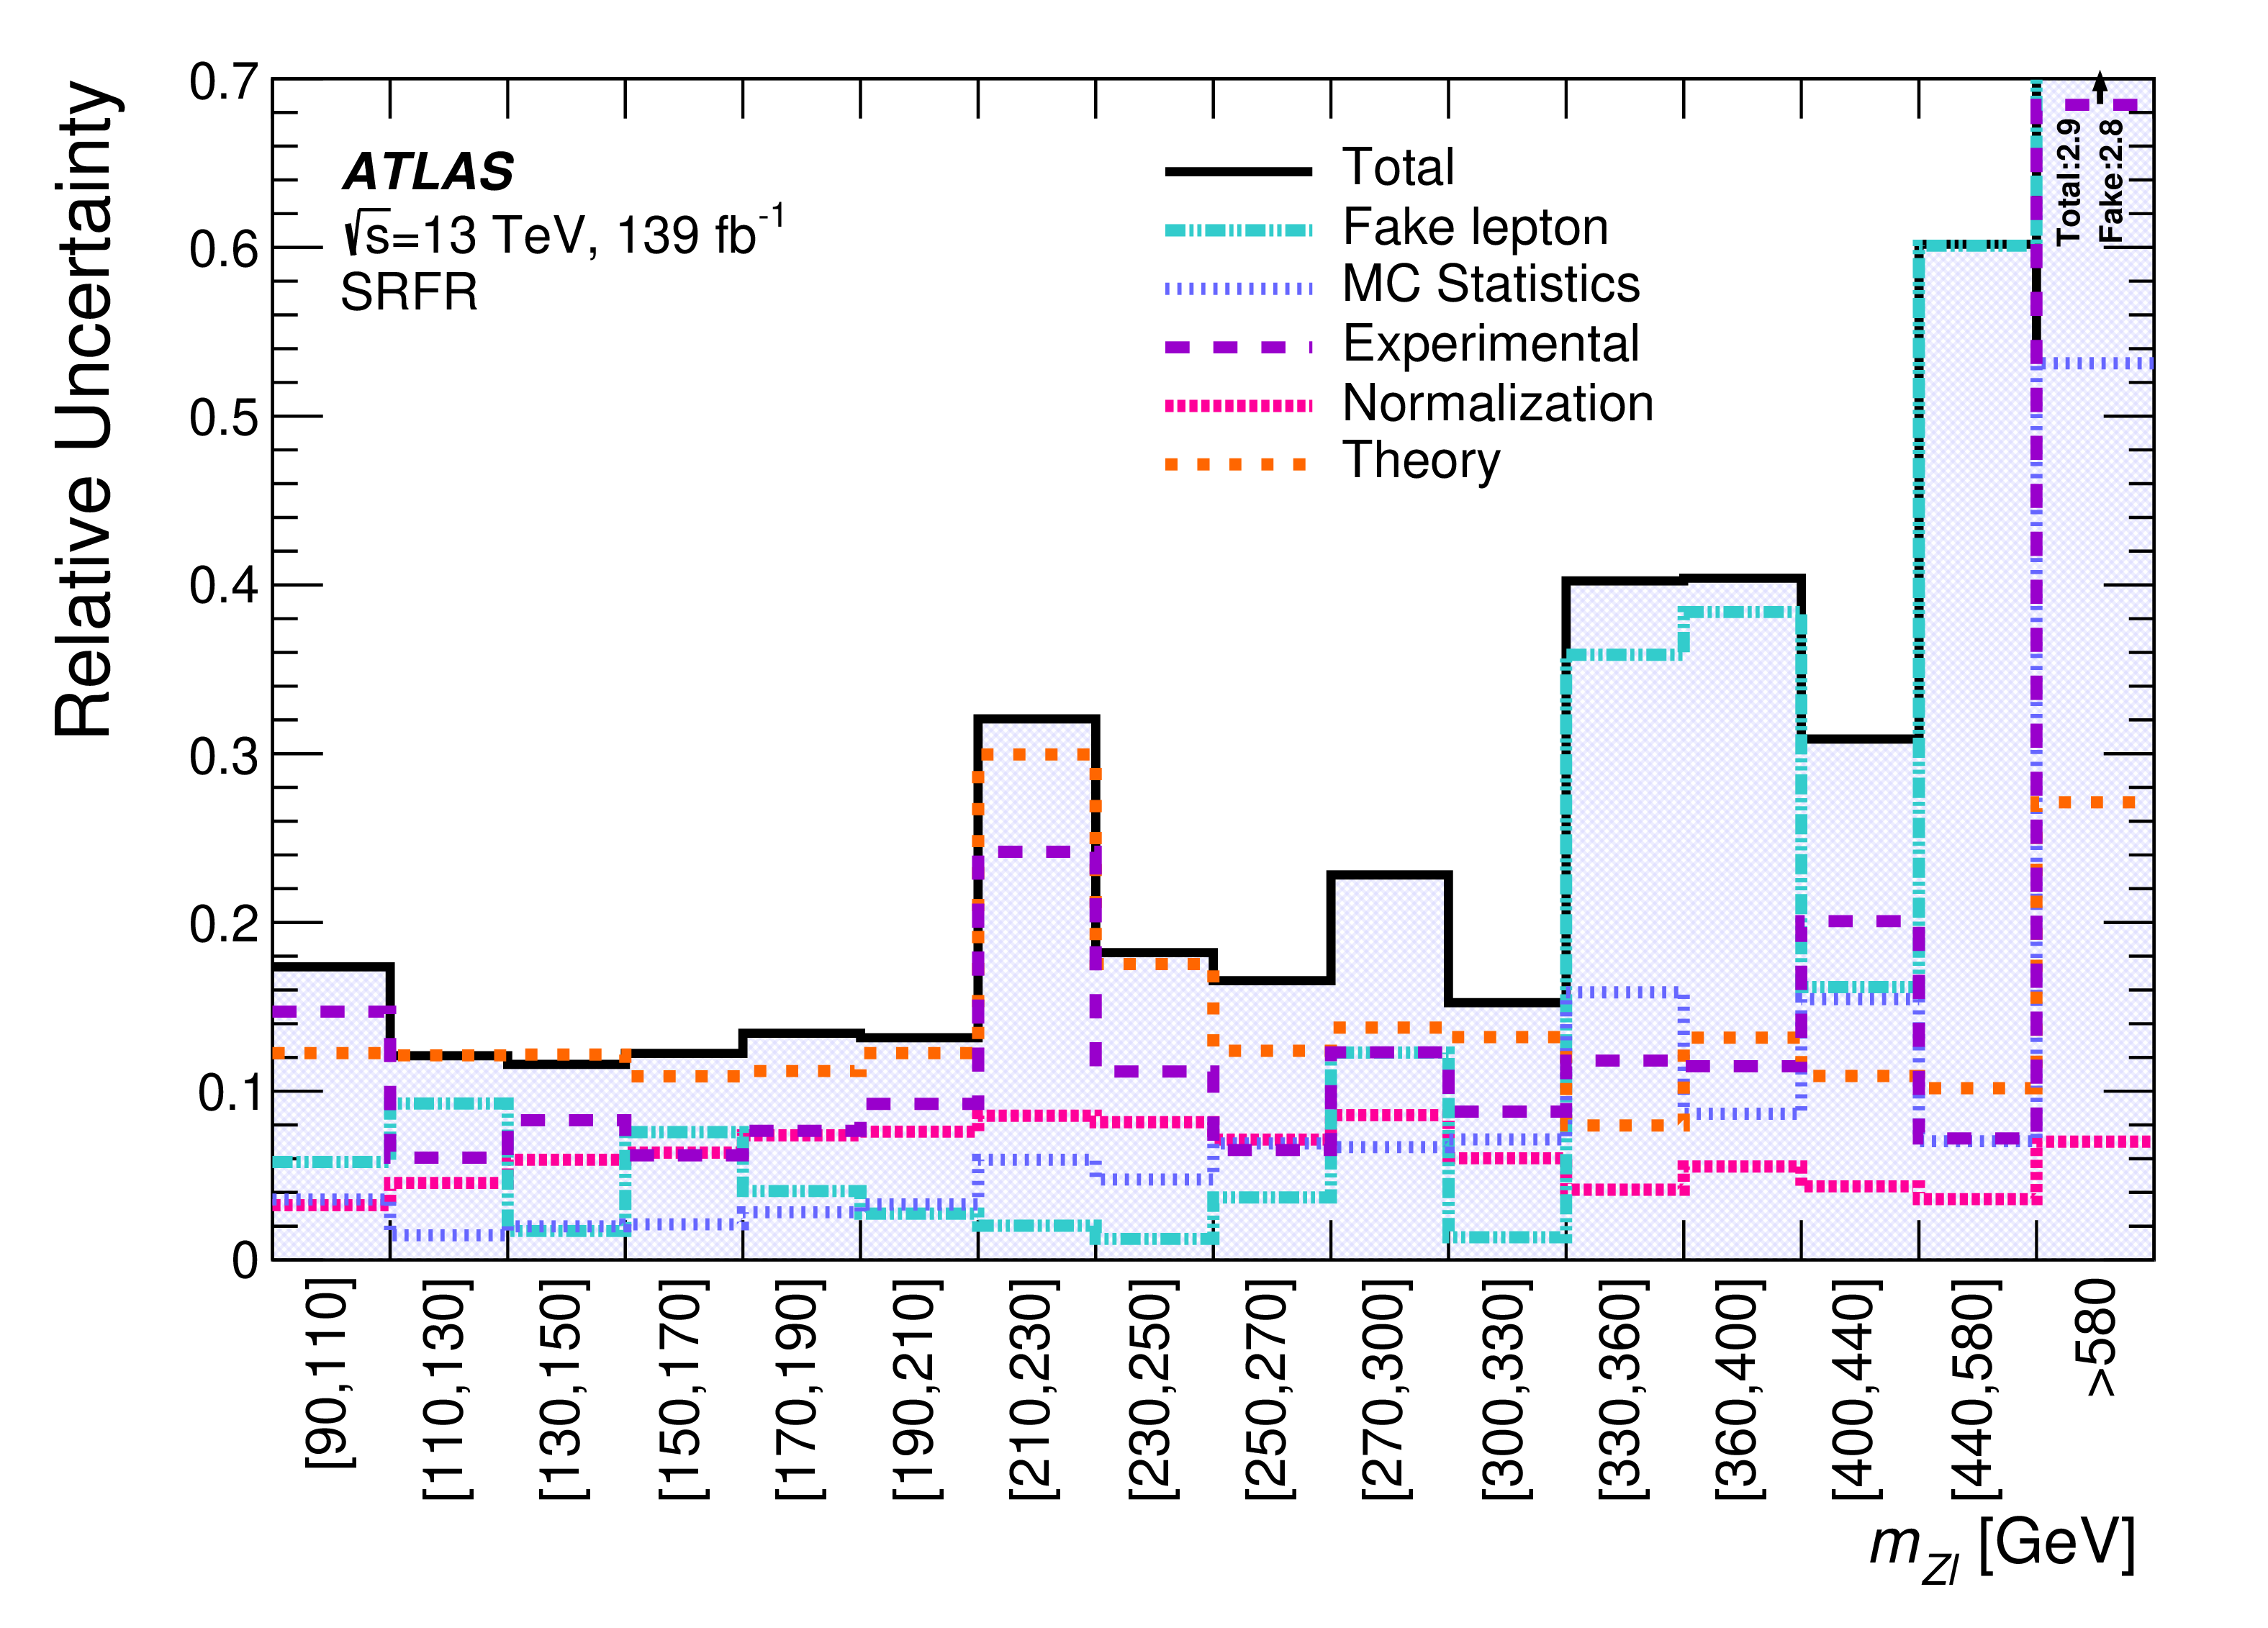
\includegraphics[width=0.98\textwidth]{figs/rpvthreel/systsflat_dist_SRTL.png}
      \caption{}
      \label{fig:systSRFR}
    \end{subfigure}
    \hfill
    \begin{subfigure}[b]{0.49\textwidth}
      \centering
      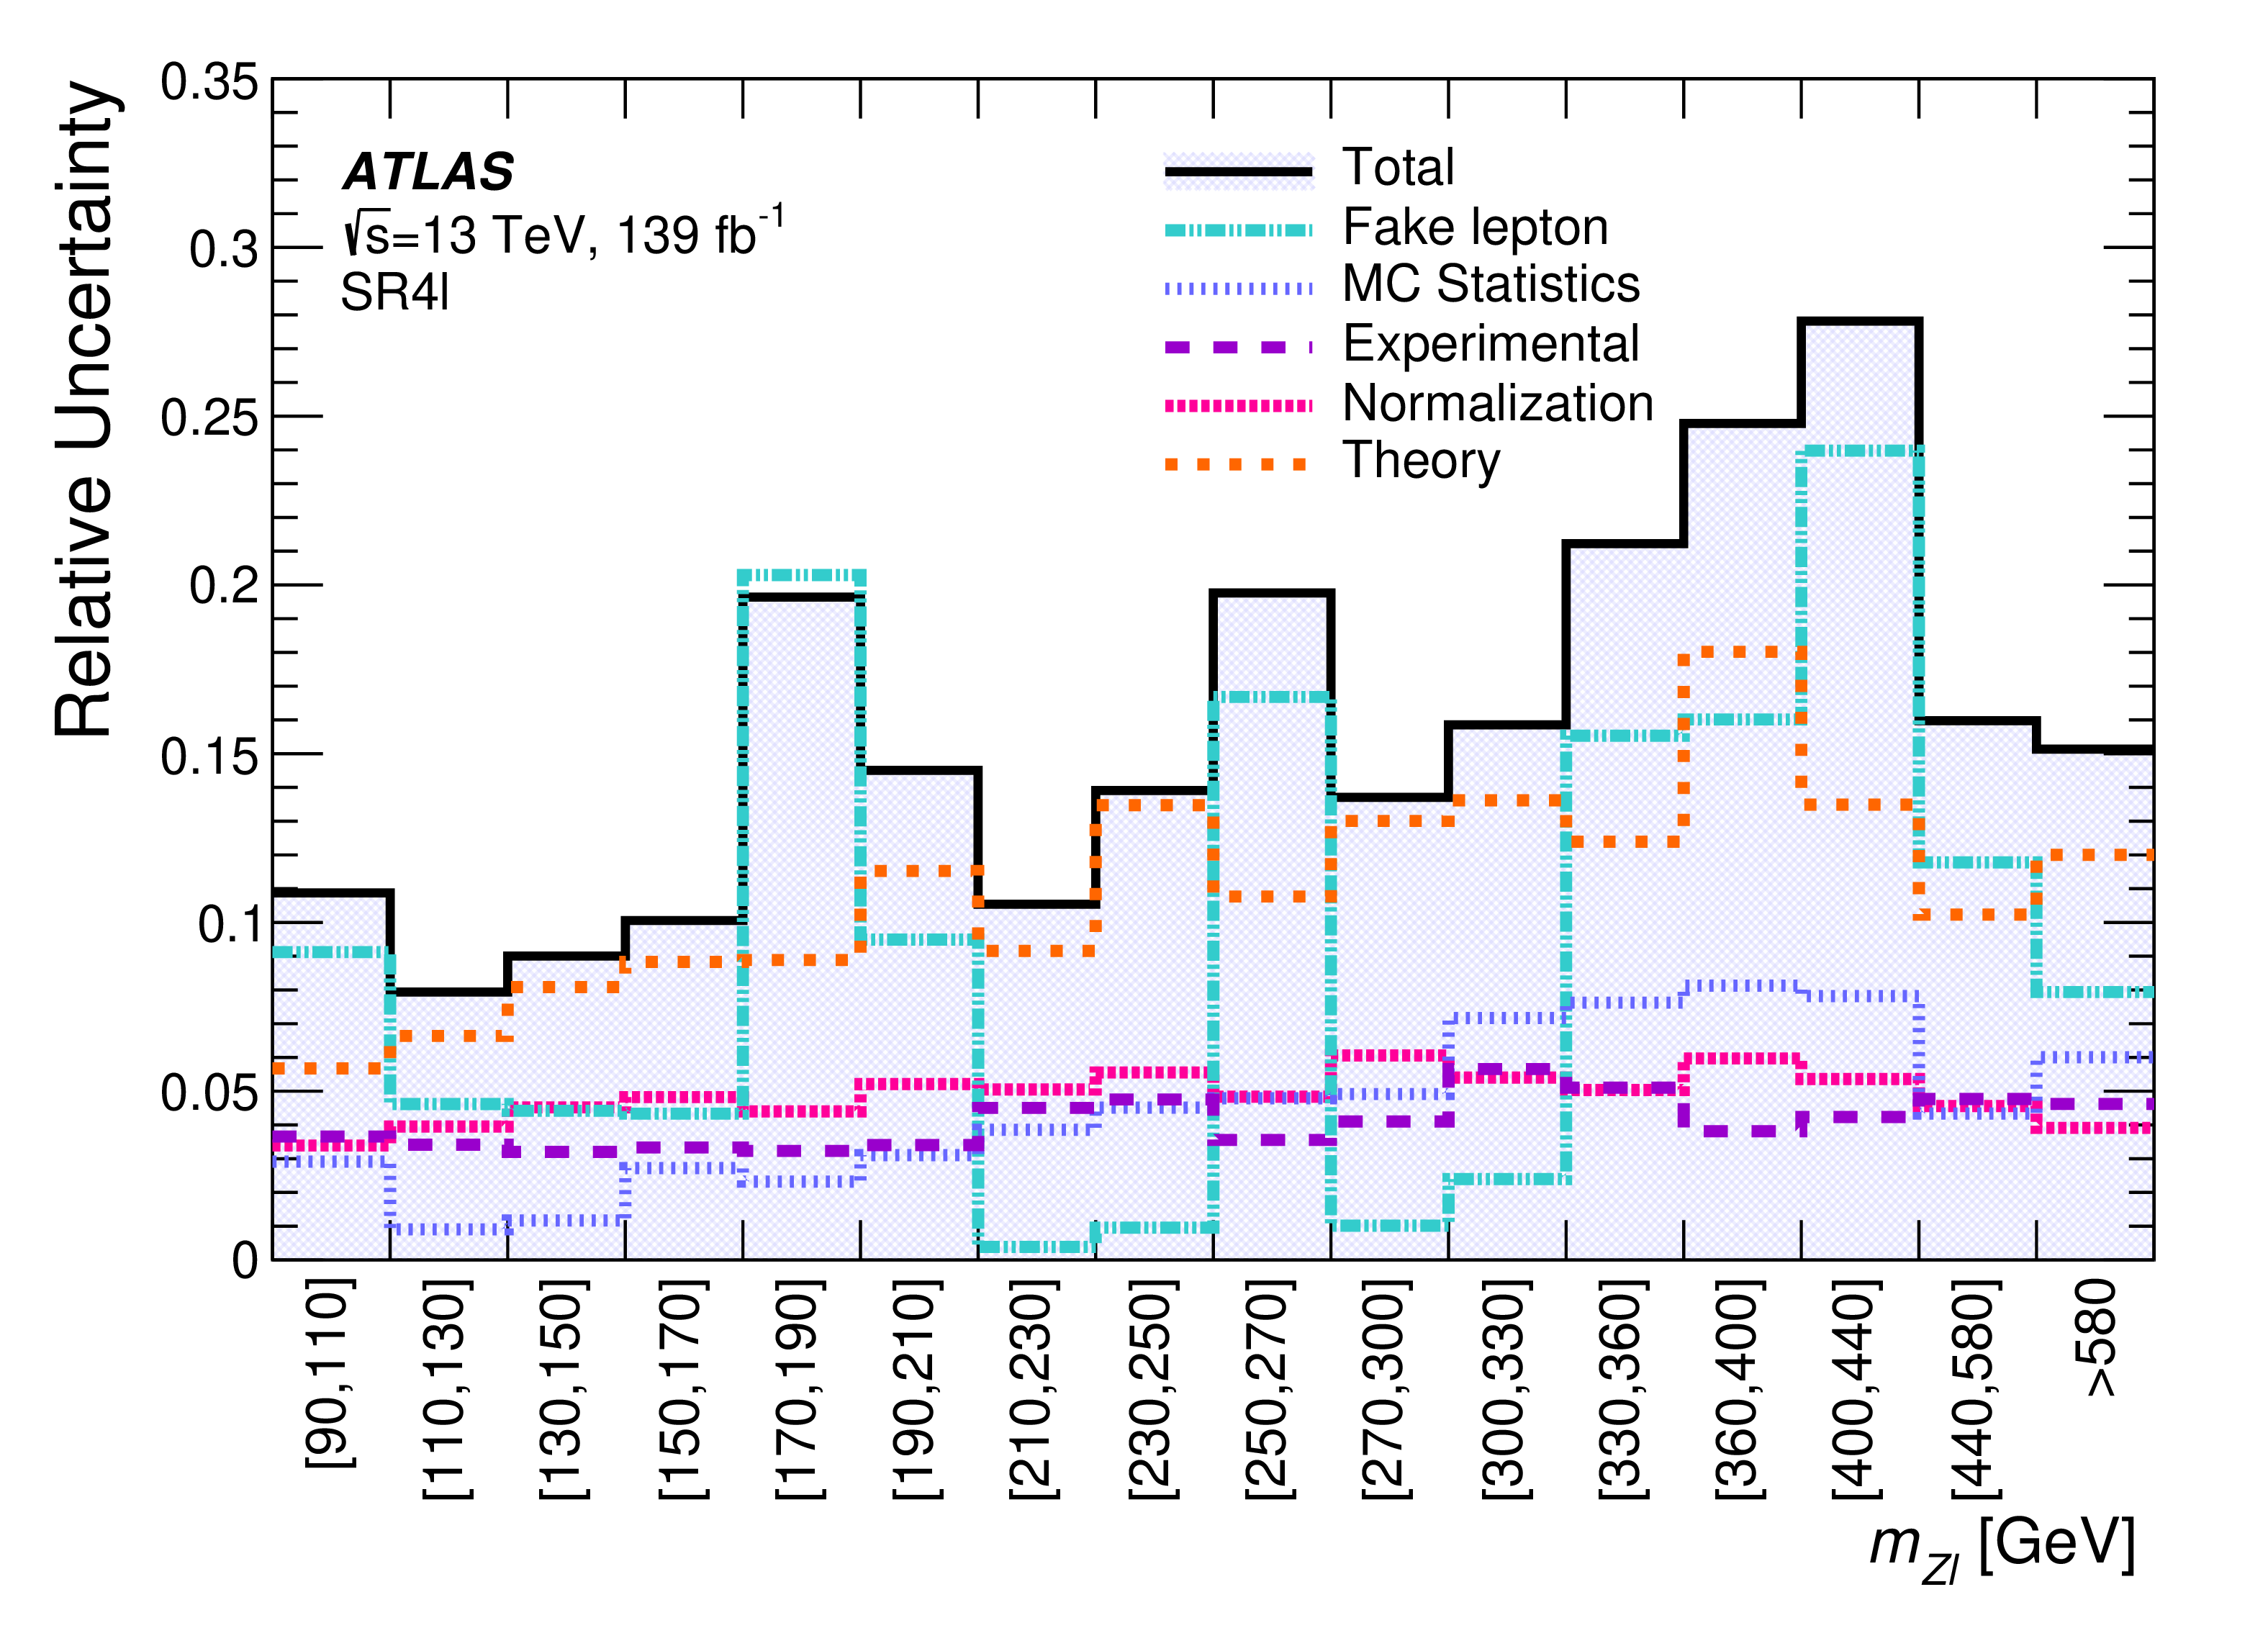
\includegraphics[width=0.98\textwidth]{figs/rpvthreel/systsflat_dist_SROL4l.png}
      \caption{}
      \label{fig:systSR4l}
    \end{subfigure}
    \hfill
    \begin{subfigure}[b]{0.49\textwidth}
      \centering
      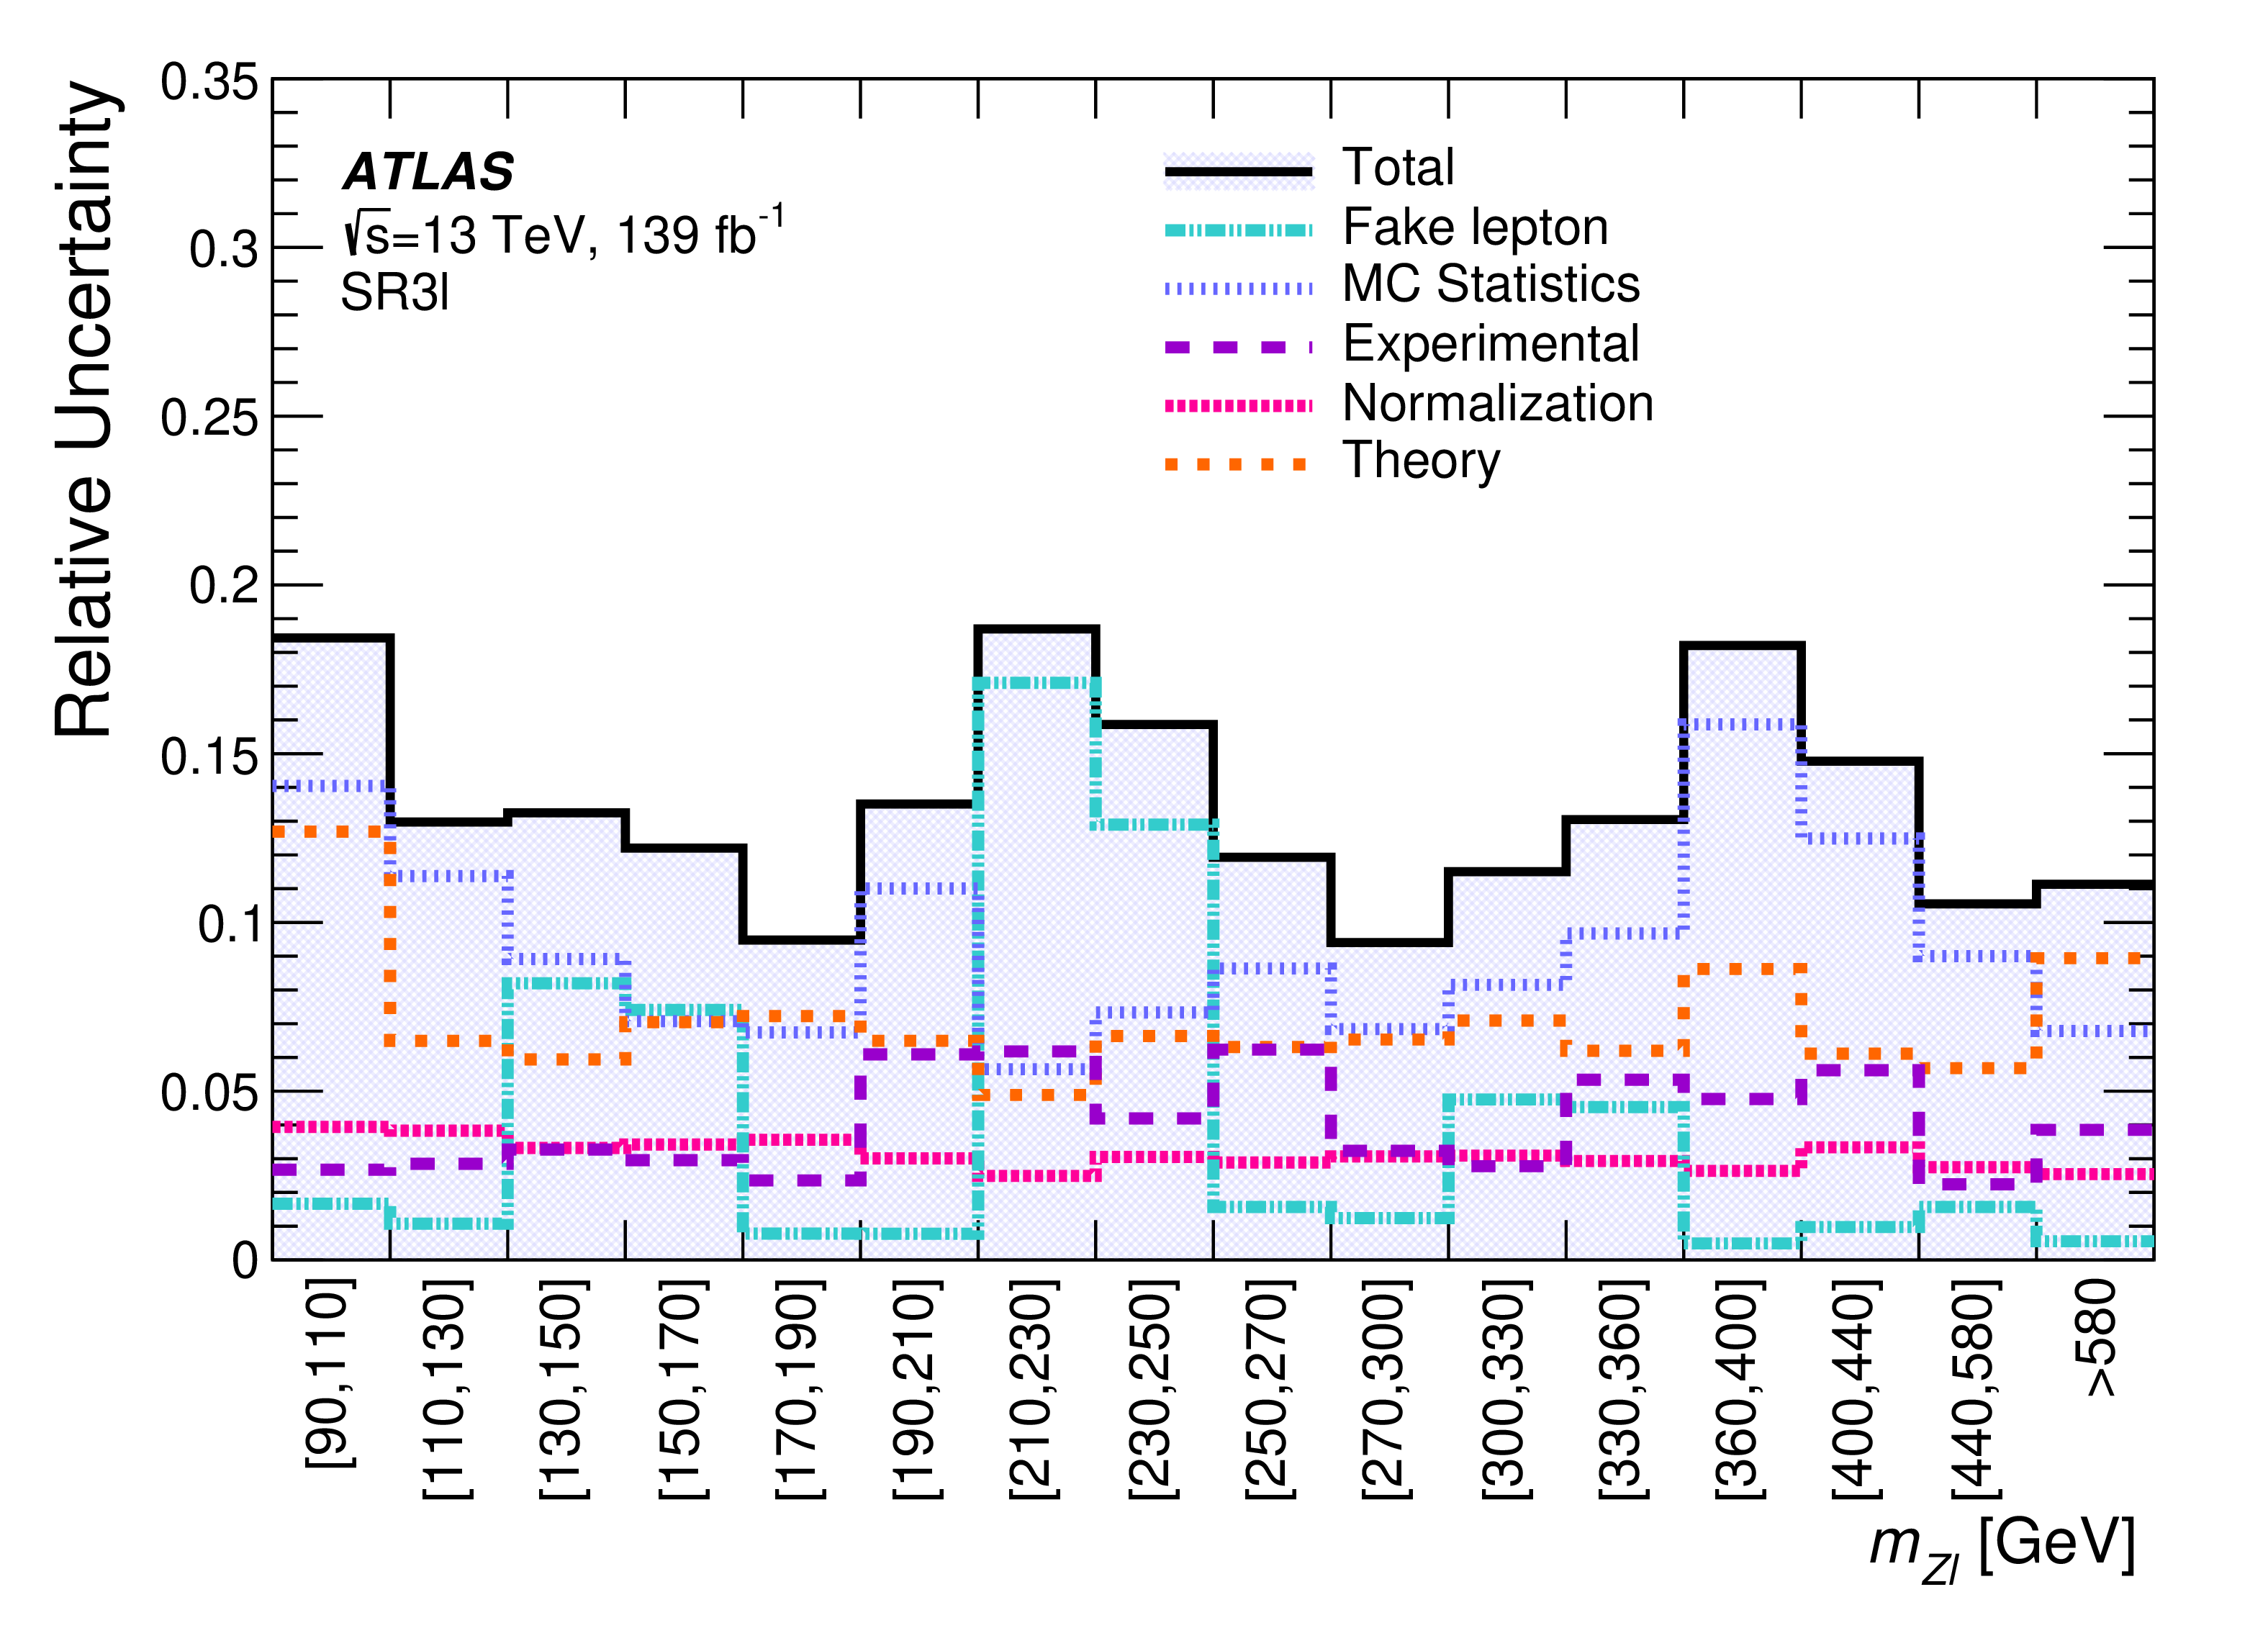
\includegraphics[width=0.98\textwidth]{figs/rpvthreel/systsflat_dist_SROL3l.png}
      \caption{}
      \label{fig:systSR3l}
    \end{subfigure}
    \caption[The relative uncertainties in the post-fit SM background prediction as a function of \mZl from the background-only fit for the (top left) \SRTL, (top right) \SRFour, and (bottom) \SRThree regions.]{The relative uncertainties in the post-fit SM background prediction as a function of \mZl from the background-only fit for the (top left) \SRTL, (top right) \SRFour, and (bottom) \SRThree regions.
    The \mZl binning (Eq.~(\ref{eq:binning})) is the same as that used in the fit.
    Sources of uncertainty are grouped into experimental, theoretical, and MC statistical categories.
    Separate categories are provided for the \fake backgrounds and for the normalization procedure of the major \WZ, \ZZ, and \ttZ backgrounds.
    The individual uncertainties can be correlated and do not necessarily contribute in quadrature to the total uncertainty \cite{ATLAS:2020uer}}
    \label{fig:systematics}
\end{figure}
\subsection{Systematic Uncertainties}
\label{sec:stats:systs}
Uncertainties in the expected signal and background yields account for the statistical uncertainties of the MC samples,
the experimental systematic uncertainties in the detector measurements, and the theoretical systematic uncertainties of the MC simulation modeling.
The uncertainties of the major backgrounds normalized in the CRs reflect the limited statistical precision of the CRs and the systematic uncertainties in the extrapolation to the signal regions, and an additional uncertainty in the normalization factor from the combined fit is included.
%The uncertainties related to the data-driven \fake background estimation are described in detail in Section~\ref{sec:background:Fake}.
Systematic uncertainties are treated as Gaussian nuisance parameters in the likelihood while the statistical uncertainties of the MC samples are treated as Poisson nuisance parameters.
A summary of the background uncertainties is shown in Figure~\ref{fig:systematics}.
Individual uncertainties can be correlated or anti-correlated, for example between an uncertainty on a major background and the uncertainty on the CR-to-SR normalization procedure for that background. 
Bin-to-bin fluctuations in the uncertainty of the \fake background estimation reflect the small anti-ID population and the conservative uncertainties applied when no anti-ID events are seen in the data.
The effect of localized fluctuations in one SR is limited as all three SRs contribute to the overall sensitivity.
A relative uncertainty of 2.9 is seen in the last \mZl bin of \SRTL and is driven by a relative uncertainty of 2.8 in the \fake estimation, reflecting the small post-fit background expectation.
A breakdown of the types of uncertainties is given in the following sections

\subsubsection{MC Statistics}
\label{sec:stats:systs:MCstats}
The nominal statistical uncertainty on the number of MC events generated makes up this category.

\subsubsection{Experimental Uncertainties }
\label{sec:stats:systs:exp}
Experimental uncertainties in the detector measurements reflect the accuracy of the kinematic measurements of jets, electrons, muons, and \met.
Varying the scale or resolution of the energy or \pt\ of objects within the uncertainties can cause the migration of events between \mZl bins or affect the inclusion of an event in an analysis region.
The jet energy scale and resolution uncertainties~\cite{PERF-2016-04,PERF-2011-04} are a large component of the experimental uncertainty. 
They are derived as a function of jet \pt\ and $\eta$ and account for the flavor and pileup dependencies of the detector energy measurement.
Similar scale and resolution uncertainties are included for electrons~\cite{EGAM-2018-01} and muons~\cite{PERF-2015-10}.
These per-object uncertainties are propagated through the \met\ calculation, with additional uncertainties accounting for the scale and resolution of the \met\ soft term~\cite{PERF-2016-07}.
Additional experimental uncertainties account for the mismodeling in MC simulation of observables related to the detection of leptons and jets.
They include the efficiency of the triggering, identification, reconstruction, and isolation requirements of electrons~\cite{EGAM-2018-01} and muons~\cite{PERF-2015-10}.
They also include the identification and rejection of pileup jets by the jet vertex tagger~\cite{PERF-2014-03} and the identification of $b$-jets by the flavor-tagging algorithm~\cite{FTAG-2018-01}.
The experimental uncertainty in the combined 2015--2018 integrated luminosity is 1.7\%~\cite{ATLAS-CONF-2019-021}, obtained primarily using the luminosity measurements of the LUCID-2 detector~\cite{LUCID2}.
Unless stated otherwise, each experimental uncertainty is treated as fully correlated across the analysis regions.

\subsubsection{Theoretical Uncertainties }
\label{sec:stats:systs:theory}
Each theoretical uncertainty is derived as the relative yield between an analysis region and a control region and is treated as uncorrelated across analysis regions.
Theoretical uncertainties in the shape of the major diboson, triboson, and \ttZ backgrounds are derived using MC simulation with varied generator parameters.
For the other minor backgrounds a conservative 20\% uncertainty is assumed.
This value is larger than is typically expected for the minor background processes and the choice has a negligible effect on the final results due to the small contributions of these backgrounds.
Uncertainties due to the choice of QCD renormalization and factorization scales~\cite{Bothmann:2016nao} are assessed by varying the relevant generator parameters up and down by a factor of two around the nominal values, allowing for both independent and correlated variations of the two scales but prohibiting anti-correlated variations.
Each QCD variation is kept separate and is treated as correlated across analysis regions.
An uncertainty of 1\% due to the chosen value of the strong coupling constant \alphas\ is assessed by varying \alphas\ by $\pm 0.001$ in the generator parameter settings.
Uncertainties related to the choice of PDF sets, CT14NNLO~\cite{Dulat:2015mca} or MMHT2014NNLO~\cite{Harland-Lang:2014zoa}, are derived by taking the envelope of the variation in event yield of 100 propagated uncertainties~\cite{Butterworth:2015oua}.

Additional theoretical uncertainties are assessed for the major backgrounds. 
These are related to assumptions made in the event generators and PS models, which can affect both the event kinematics and the cross section of the physics process.
For the diboson backgrounds, the \SHERPA parameters related to the PS matching scale and resummation scale are varied up and down by a factor of two around the nominal values, and an alternative recoil scheme is studied.
For the \ttZ background, the uncertainties in the hard scatter and in the PS are derived through a comparison with the \SHERPA and \amchseven predictions, respectively.
Additional uncertainties in the amount of initial-state radiation (ISR) in the \ttZ background are assessed by varying the related generator parameters.

For the signal samples, theoretical uncertainties in the cross section are applied, ranging from 4.5\% at 100~\GeV to 16\% at 1500~\GeV.
Uncertainties related to the QCD scale, PS matching scale, and amount of ISR are derived by varying the related generator parameters of the A14 tune~\cite{ATL-PHYS-PUB-2014-021}.

\subsubsection{Fake Lepton Uncertainties}
\label{sec:stats:systs:fakes}
Alternative parameterizations to the nominal \ptcone are used to define a systematic uncertainty due to the choice of \ptcone ~\cite{ATLAS:2020uer}.
The statistical uncertainty of each \fake factor is propagated to an uncertainty in the yield.
An uncertainty due to the prompt-lepton subtraction is estimated by varying the subtracted yields of the \WZ and \ZZ MC simulations up and down by 5\%, corresponding to their cross-section uncertainties~\cite{STDM-2018-03}.
For any \mZl bin of an SR that does not have an anti-ID event, and therefore has a prediction of zero \fake-lepton events, an uncertainty is applied corresponding to a yield of 0.32 \fake events.
This represents the largest \fake estimate possible given a 1 sigma upward fluctuation in the anti-ID event yield.

\subsubsection{Normalization Uncertainties}
\label{sec:stats:systs:normalization}
These are the uncertainties on the normalization factors $\mu_{t\bar{t}Z}$, $\mu_{
WZ}$, and $\mu_{ZZ}$ and are determined from the fit and dominated by the statistics in the control regions.



\subsection{Fit Configuration}
%The simultaneous fit accounts for any expected contributions in the control regions due to the target signal model.
%First estimates of the expected background contributions are extracted from MC estimates.
%The various background processes were grouped as described in \ref{sec:regions}.
%The normalization for the \WZ, \ZZ, and \ttZ samples are allowed to float when performing the fit, while the normalization for the other background processes are fixed to their theoretical cross-section, with the exception of our reducible backgrounds (primarily \Zjet) which are estimated via the fake factor method as described in \ref{sec:fakes}.
The \Histfitter package~\cite{Baak:2014wma}, version 0.62.0, is used to perform the simultaneous fit of the control and signal regions.
\Histfitter is a flexible statistical tool used in many ATLAS SUSY analyses.
For each process, a \texttt{ROOT}~\cite{ROOT} tree is created containing all the kinematic quantities and weights used in the analysis.
The signal, control, and validation regions are then defined within the \Histfitter configuration file to select events which are to be considered.

\subsection{Background-Only Fit}
\label{sec:stats:bkgonly}
The first fit we will consider is the so called ``background only fit.''
This fit's purpose is two fold, and takes on two different flavors as a result.
The first flavor includes only the control regions, this is the very first fit done in order done to verify that the background prediction can model the data in the CRs and VRs, where the signal contamination in is negligible, such that the SRs can be unblinded.
Once this initial fit is done, and an initial set of parameters estimated, the SRs are unblinded.
Only after unblinding can the second flavor of the fit be performed.
In this fit \emph{both} CRs and SRs are all fit simultaneously in order to make physics statements.
This fit results in the final values for the normalization factors which are shown in Table~\ref{tab:normfactors}.
For both flavors of this fit $\mu_{sig}$ in Equation \ref{eq:statmodel} is set to zero.
For the CR only we of course take $i$ to be $i$ = \CRttZ, \CRWZ, \CRZZ and for the CR+SR fit $i$ remains unchanged from Equation \ref{eq:statmodel}.
Several kinematic distributions are shown for the CRs and VRs post-fit in Figure~\ref{fig:postfitkinematics}.
The data-MC agreement for the yields in the CRs (pre-fit) and VRs (post-fit) is shown in Figure~\ref{fig:dataMCagreement_CRVR}.
The data agree well with the post-fit background estimates in all validation regions, giving confidence in the validity of the post-fit background estimation in the SRs.
A slight overestimation of almost $2\,\sigma$ is seen in \VRmet, and no features are seen in the comparison of data and the post-fit background estimates in the \mZl (Figure~\ref{fig:mZl}) or \met (Figure~\ref{fig:Nminus1VRMet}) distributions of \VRmet.
A minor excess of data over the background estimation of $1.3\,\sigma$ is seen in \VRttZ, and good agreement is seen in the shape of the relevant \mZl (Figure~\ref{fig:mZl}) and \dRbb (Figure~\ref{fig:Nminus1CRttZ}) distributions.

\begin{table}[h]
    \centering
    \begin{tabular}{c|c}
    \toprule
         $\mu_{WZ}$ & $1.01\pm0.03$ \\
         \midrule
         $\mu_{ZZ}$ & $1.12\pm0.06$ \\ 
         \midrule
         $\mu_{t\bar{t}Z}$ & $1.05\pm0.18$ \\ 
         \bottomrule
    \end{tabular}
    \caption{MC normalization factors for major backgrounds.}
    \label{tab:normfactors}
\end{table}

\begin{figure}
    \centering
    \begin{subfigure}[b]{0.49\textwidth}
      \centering
      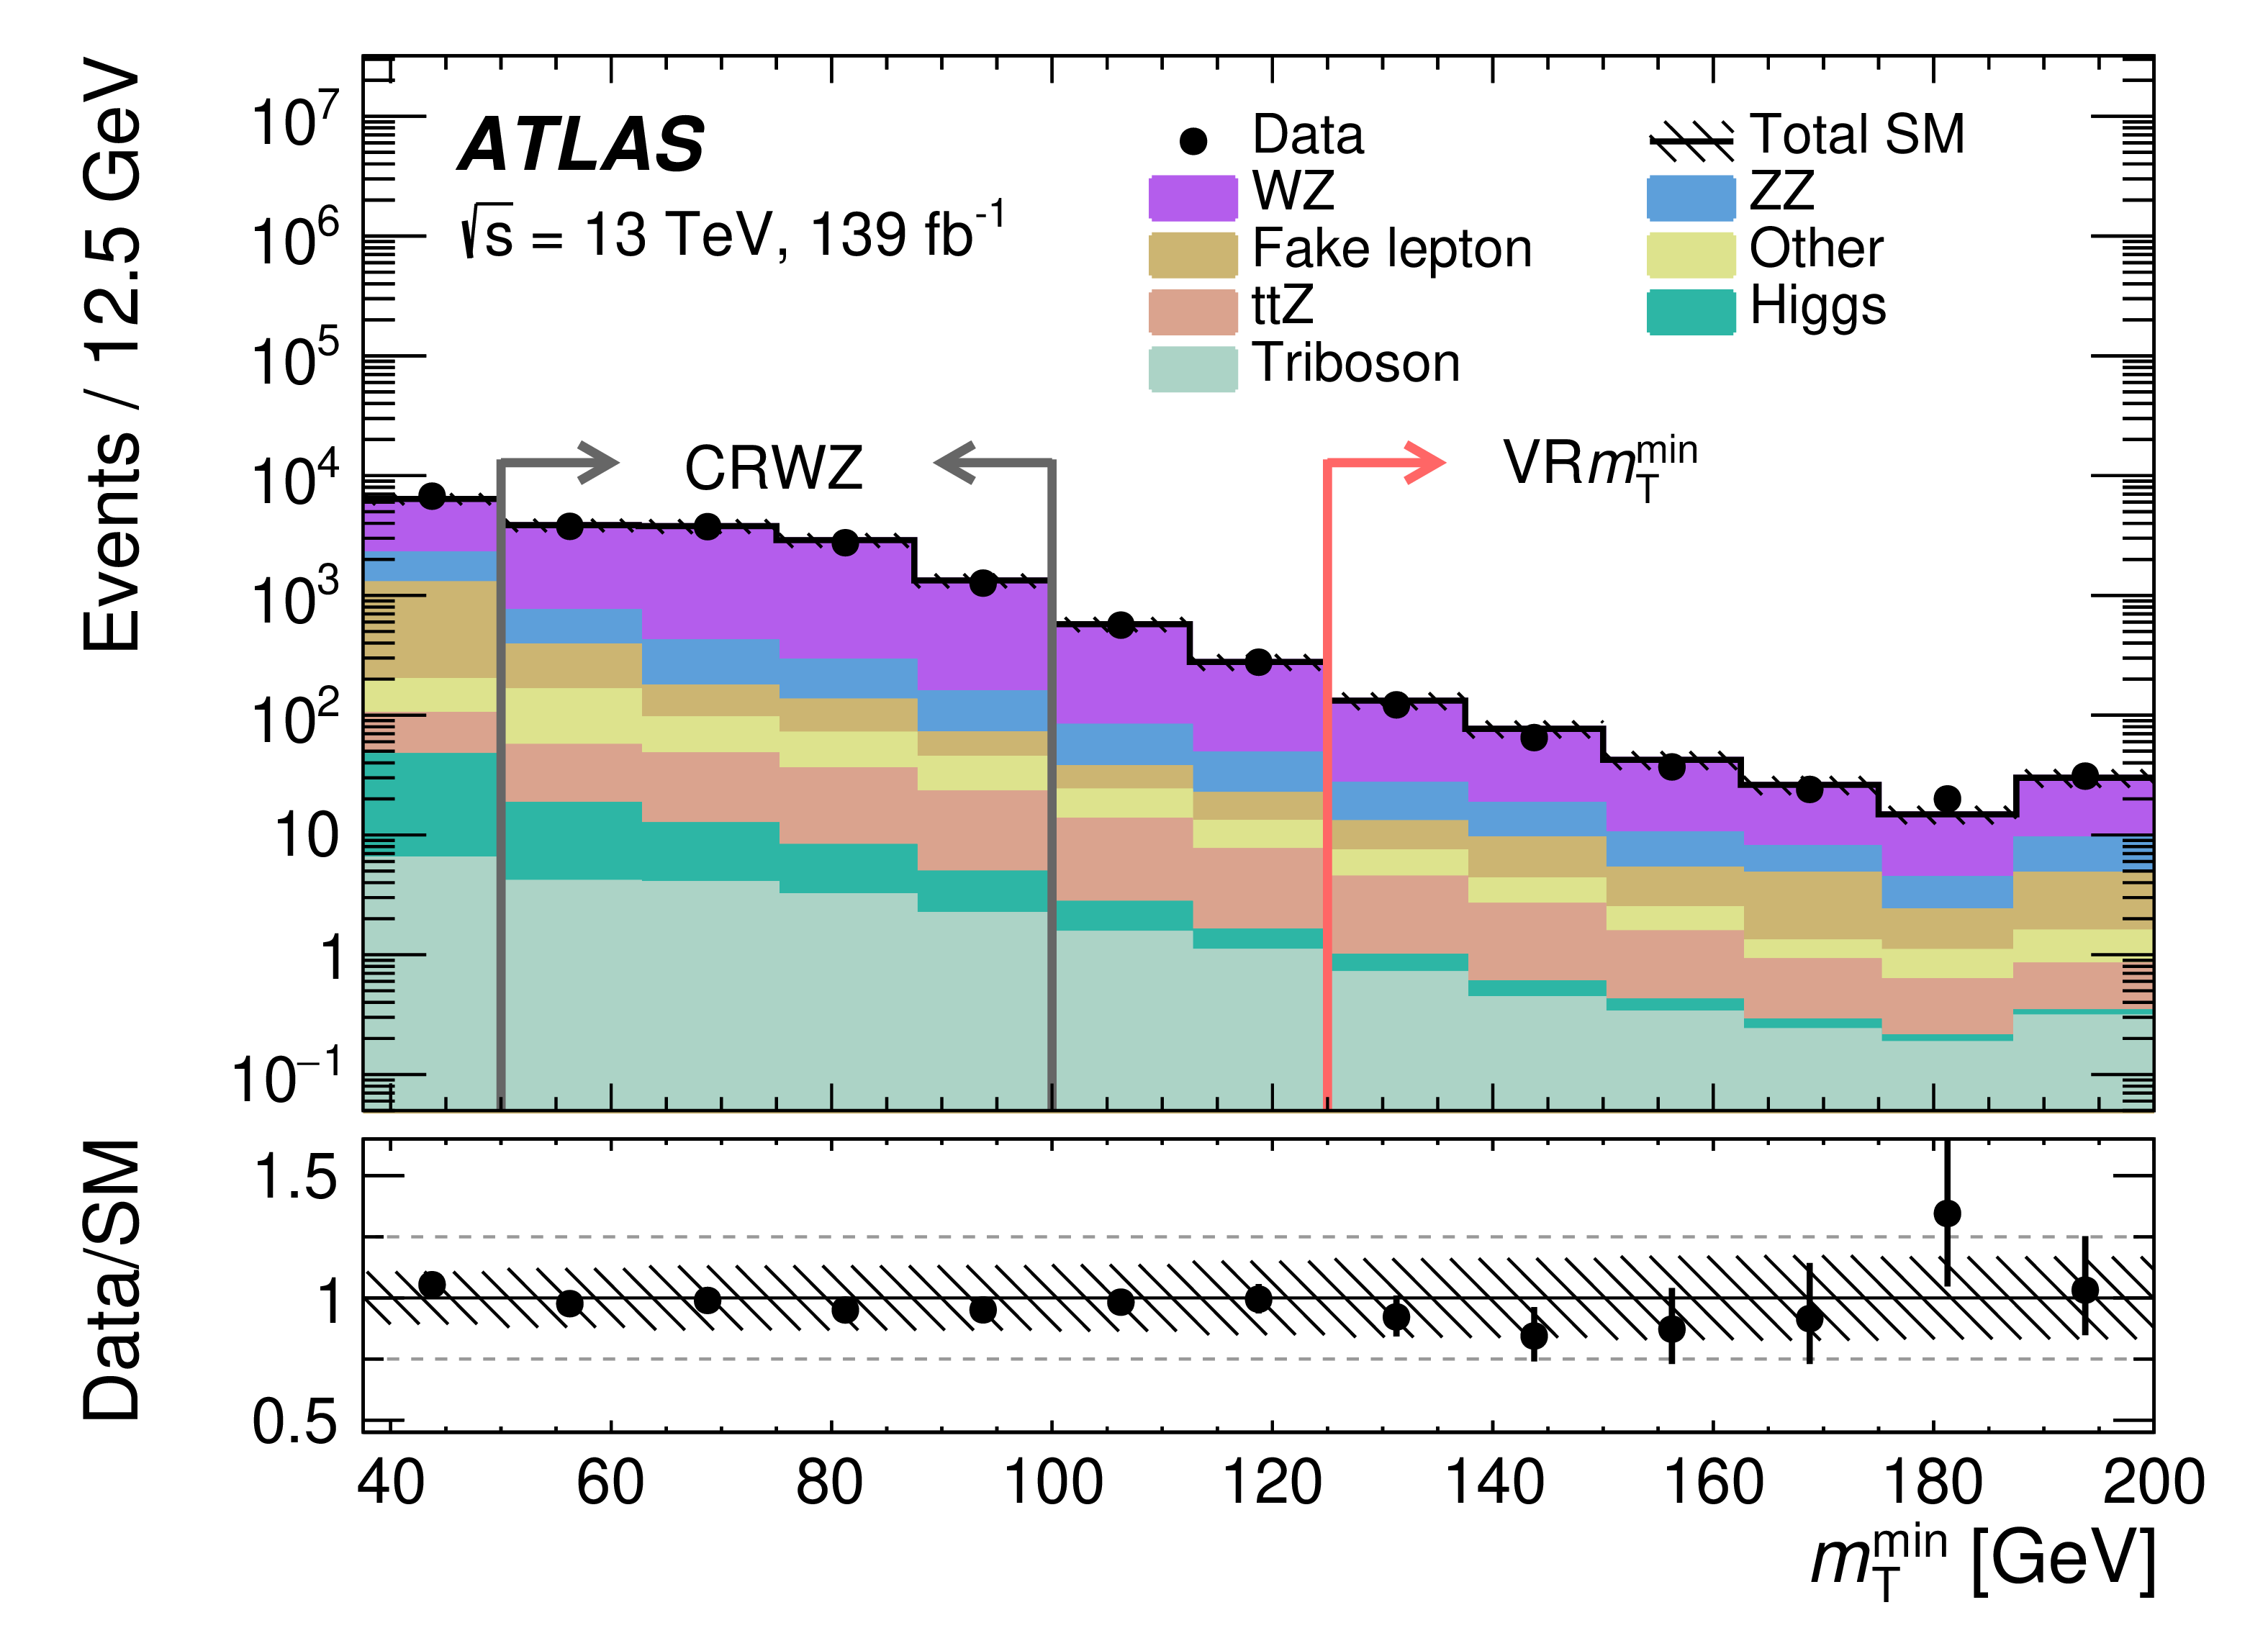
\includegraphics[width=0.98\textwidth]{figs/rpvthreel/CRWZ_Nm1_mTmin_logy.png}
      \caption{}
      \label{fig:Nminus1CRWZmTmin}
    \end{subfigure}
    \hfill
    \begin{subfigure}[b]{0.49\textwidth}
      \centering
      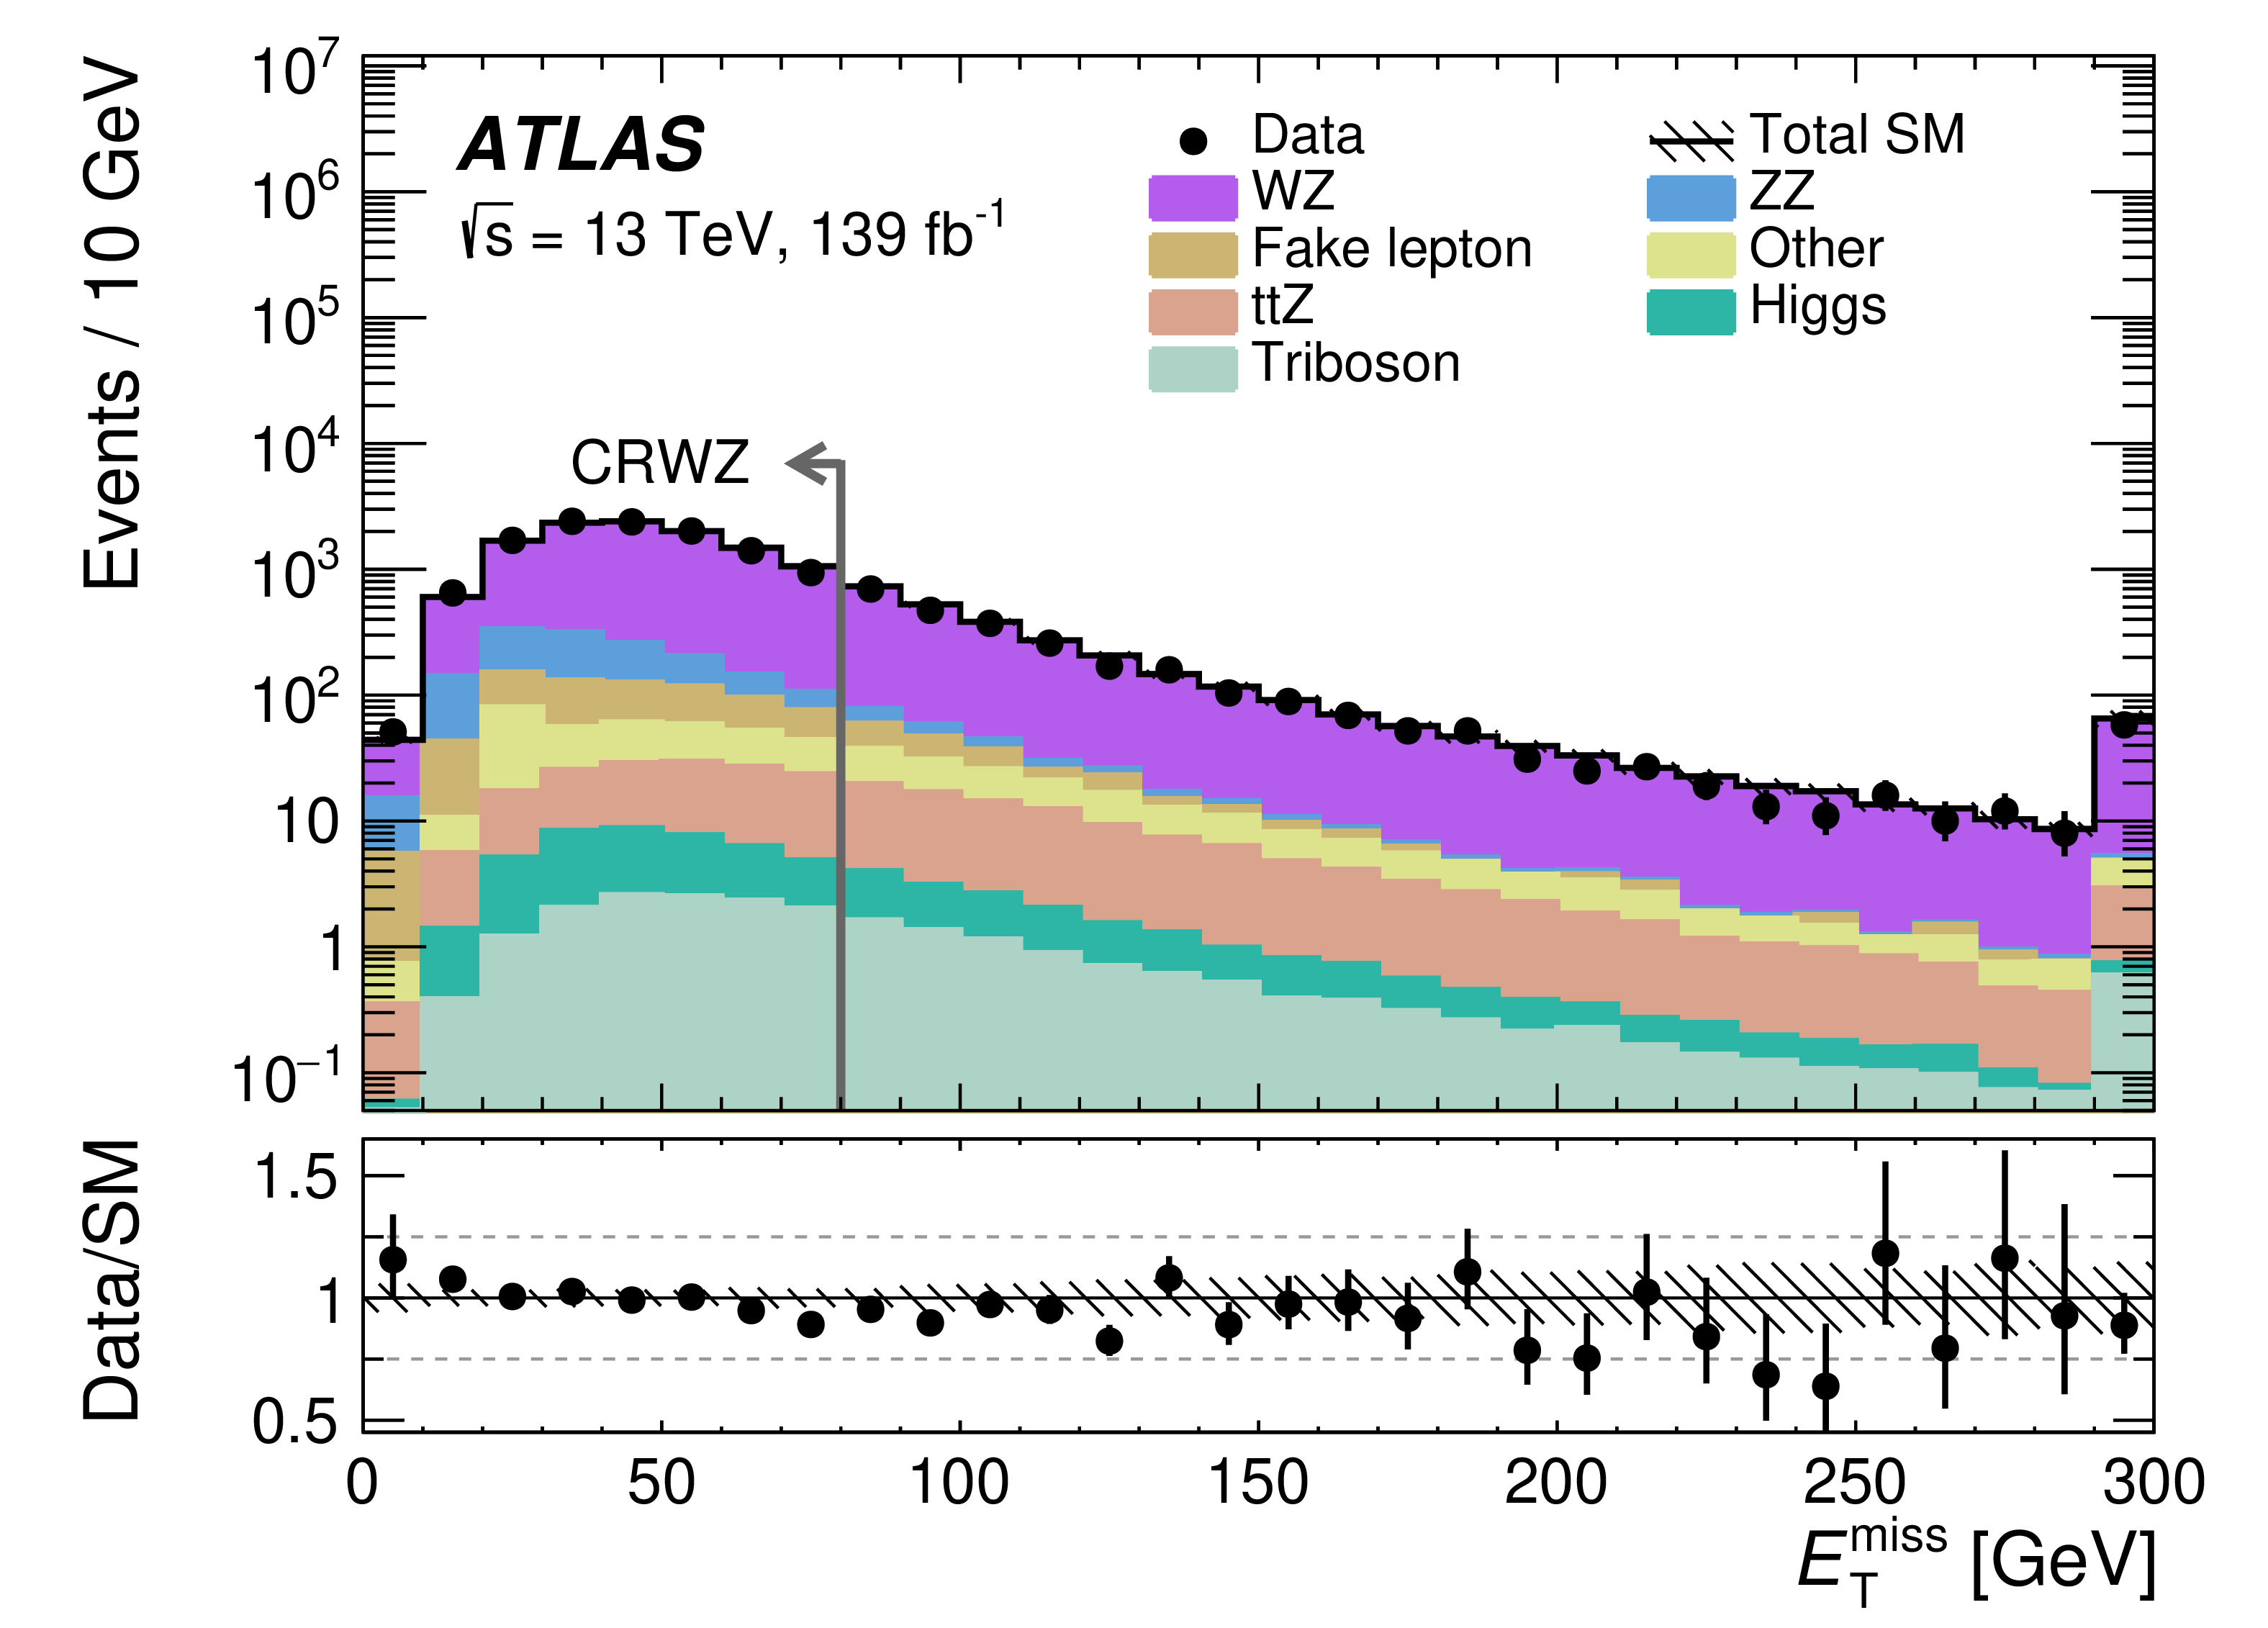
\includegraphics[width=0.98\textwidth]{figs/rpvthreel/CRWZ_Nm1_met_logy.png}
      \caption{}
      \label{fig:Nminus1CRWZmet}
    \end{subfigure}
    \hfill
    \begin{subfigure}[b]{0.49\textwidth}
      \centering
      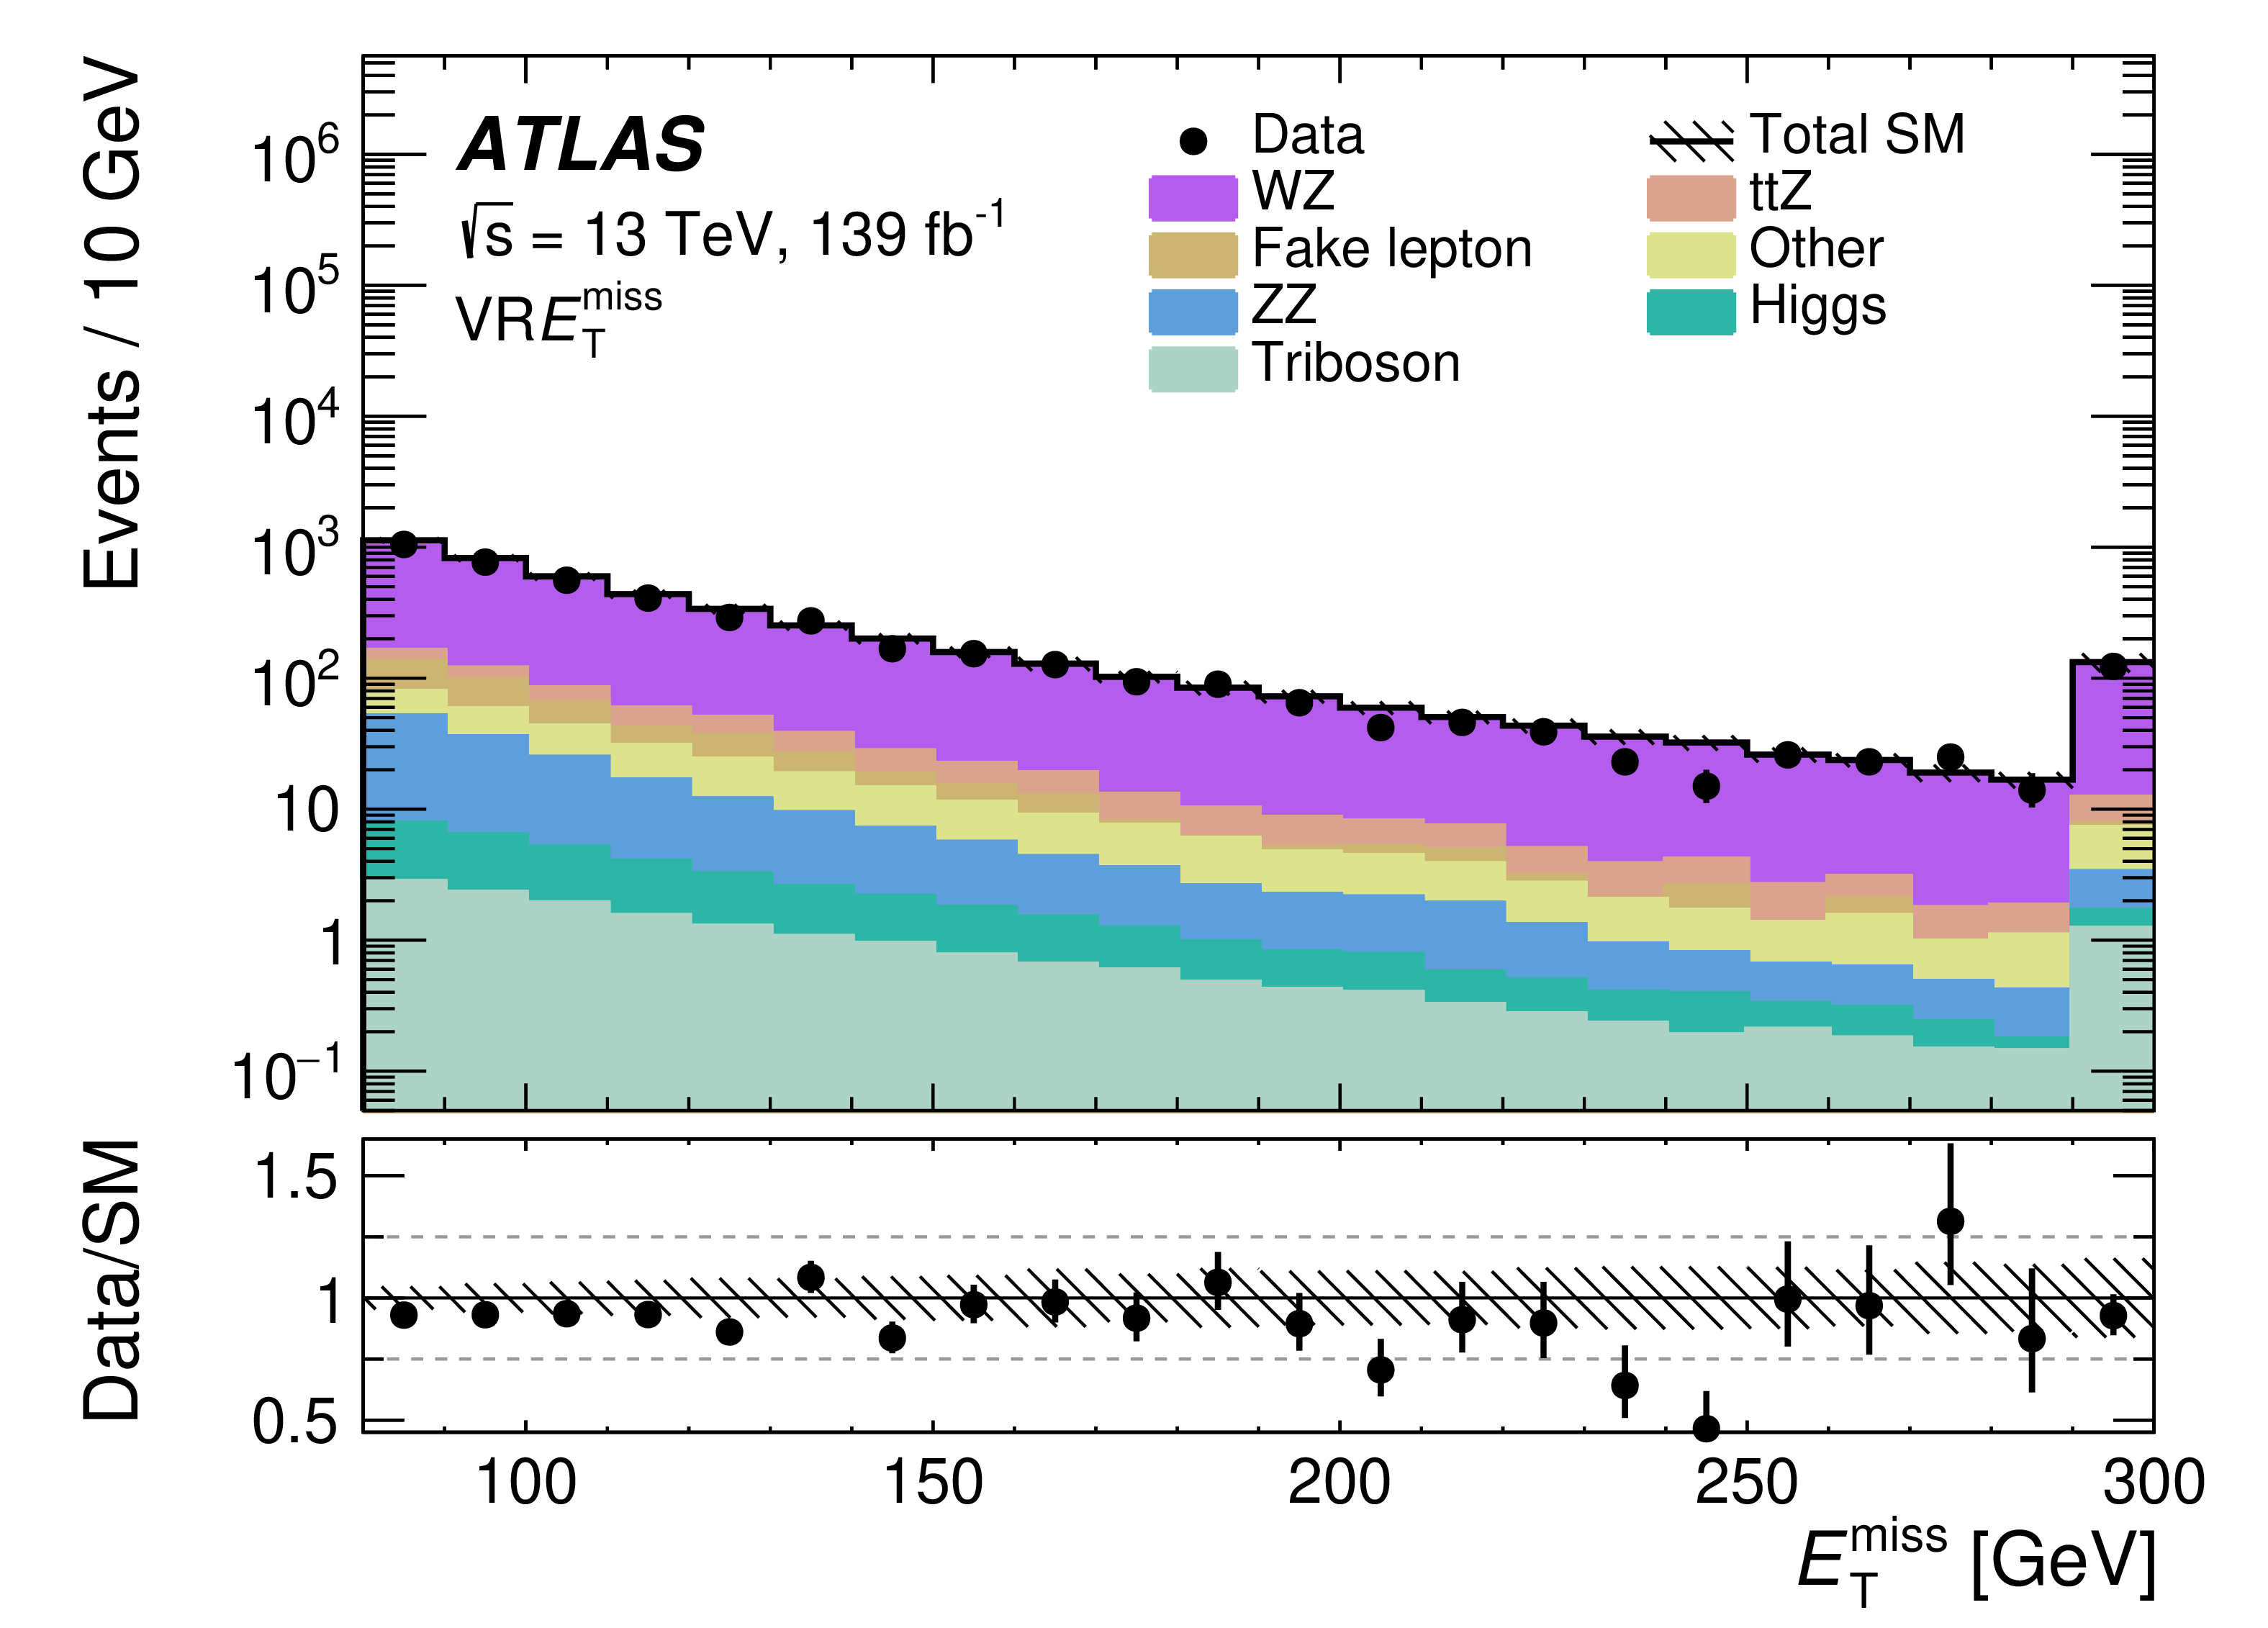
\includegraphics[width=0.98\textwidth]{figs/rpvthreel/VRMet_met_logy.png}
      \caption{}
      \label{fig:Nminus1VRMet}
    \end{subfigure}
    \hfill
    \begin{subfigure}[b]{0.49\textwidth}
      \centering
      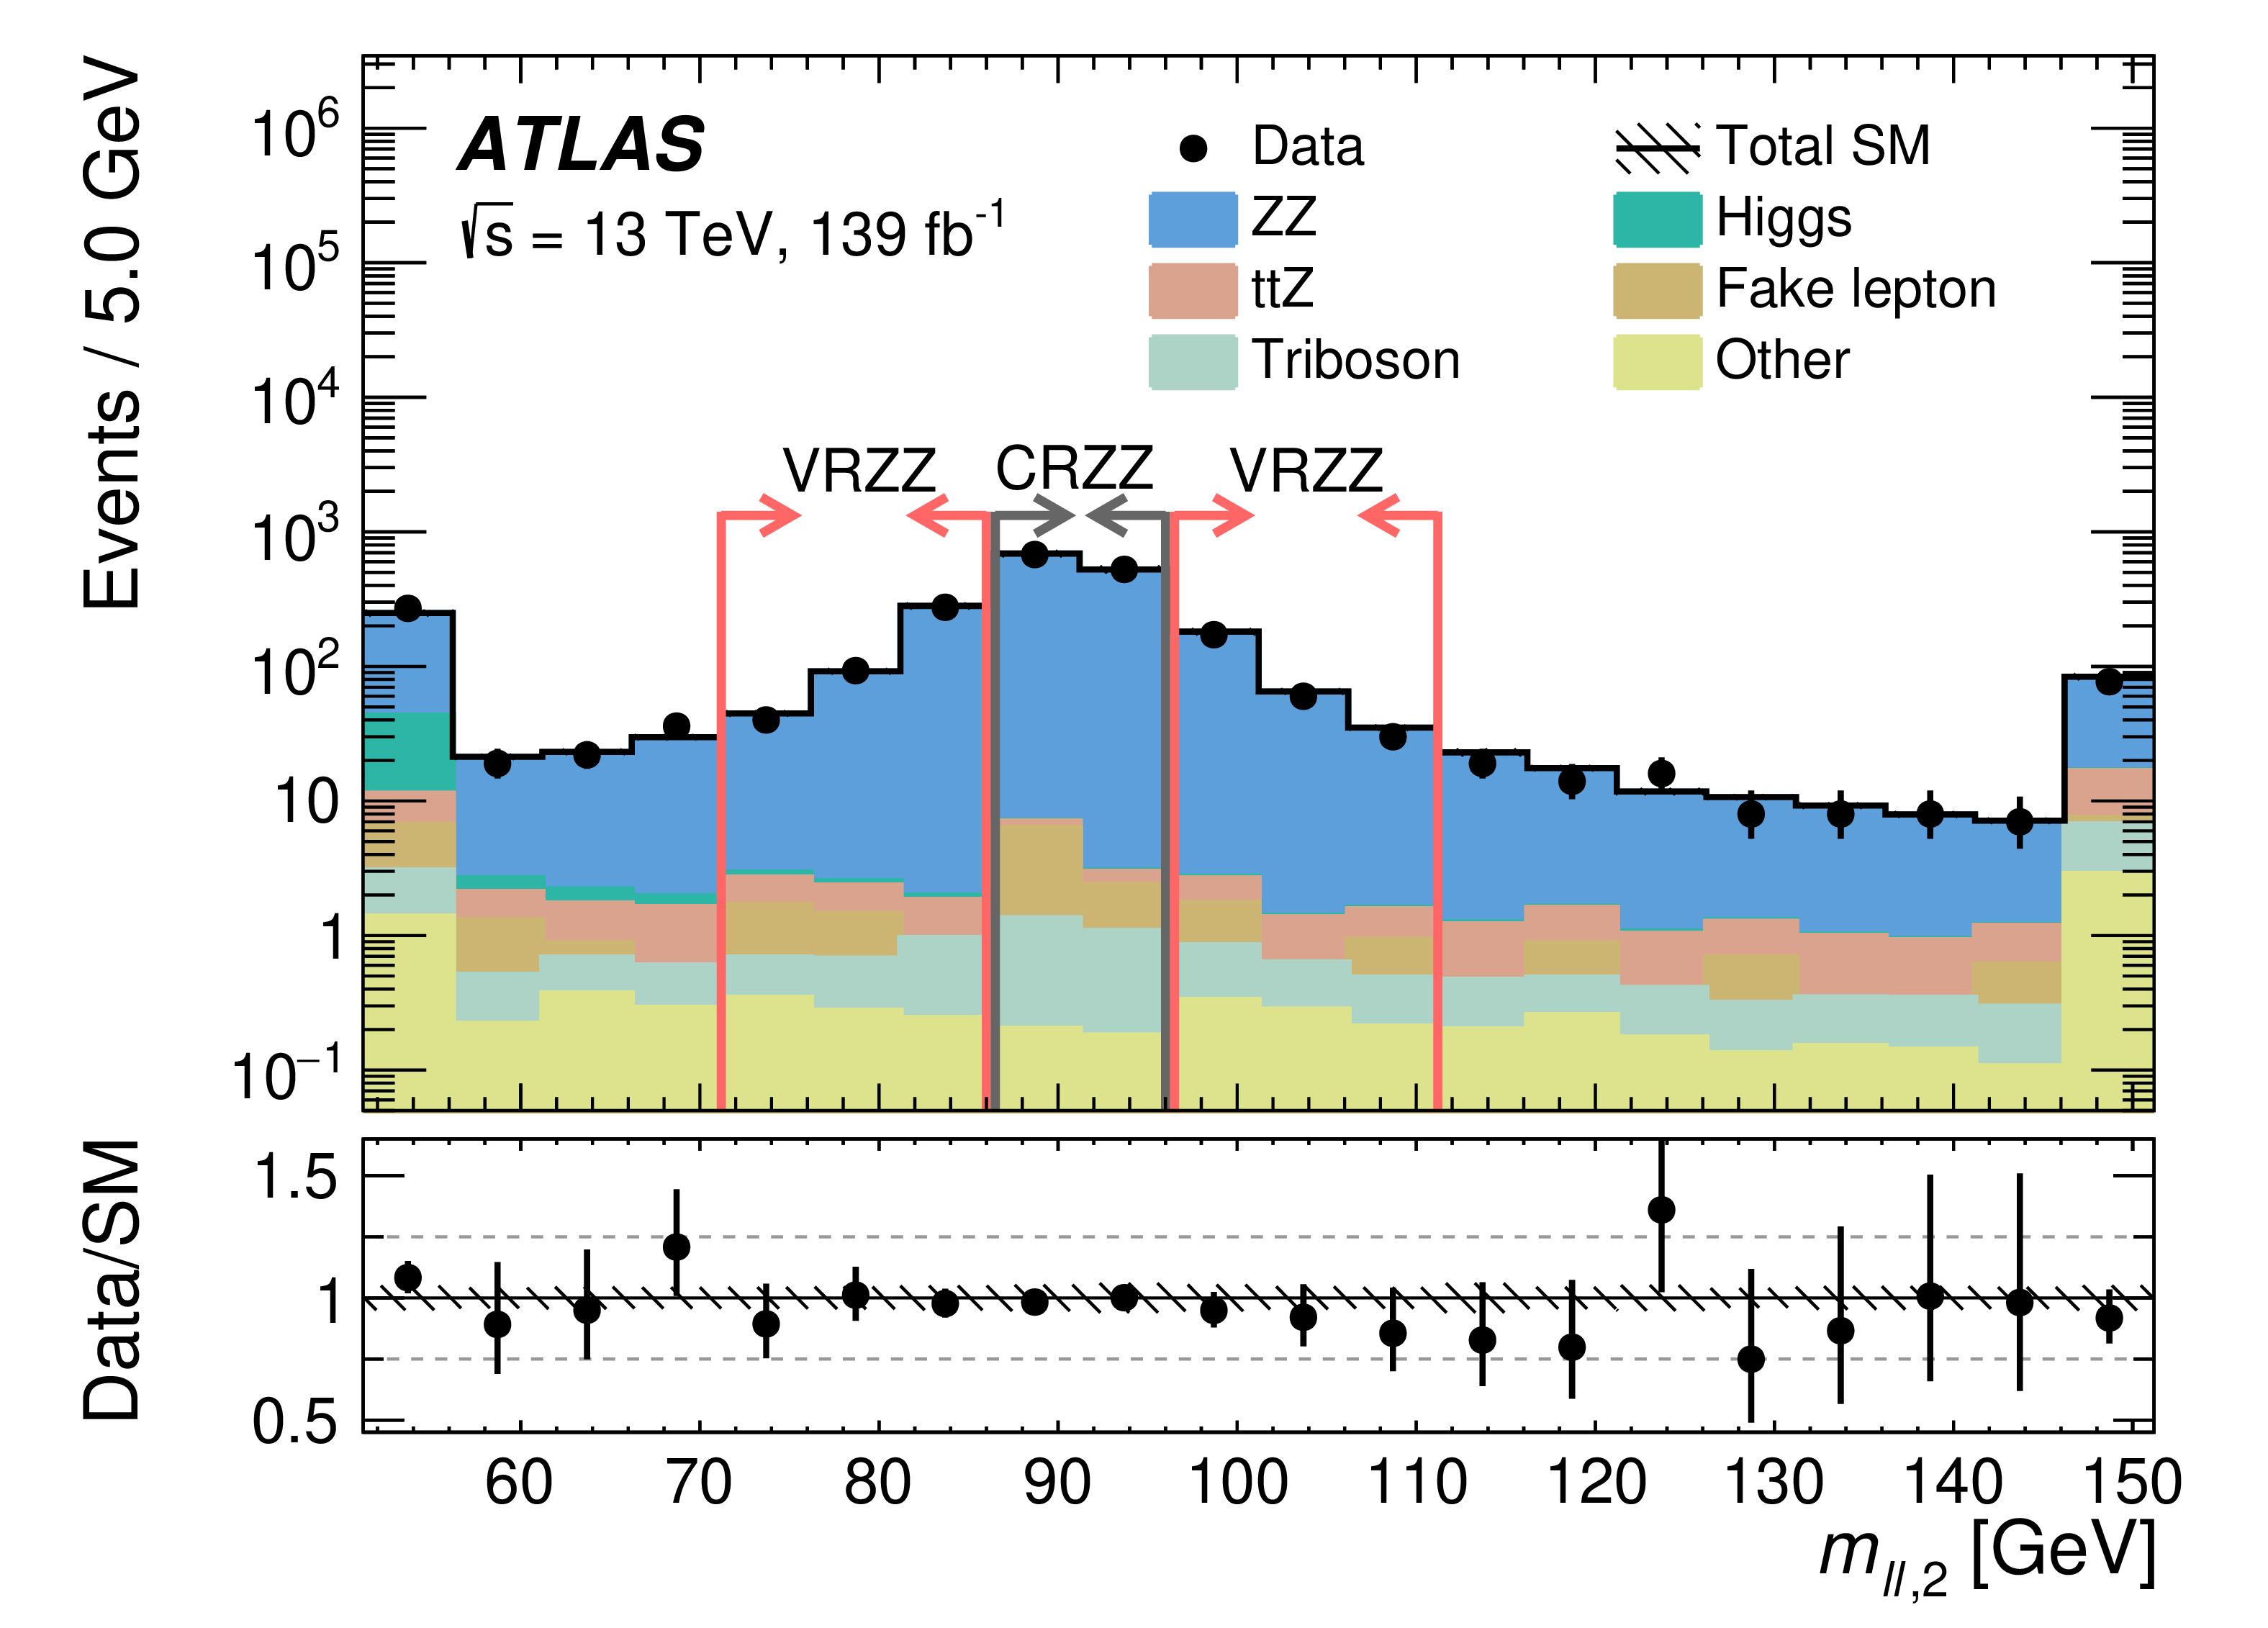
\includegraphics[width=0.98\textwidth]{figs/rpvthreel/CRZZ_Nm1_m_allLeptonicZs_1_logy.png}
      \caption{}
      \label{fig:mll2ZZ}
    \end{subfigure}
    \hfill
    \begin{subfigure}[b]{0.49\textwidth}
      \centering
      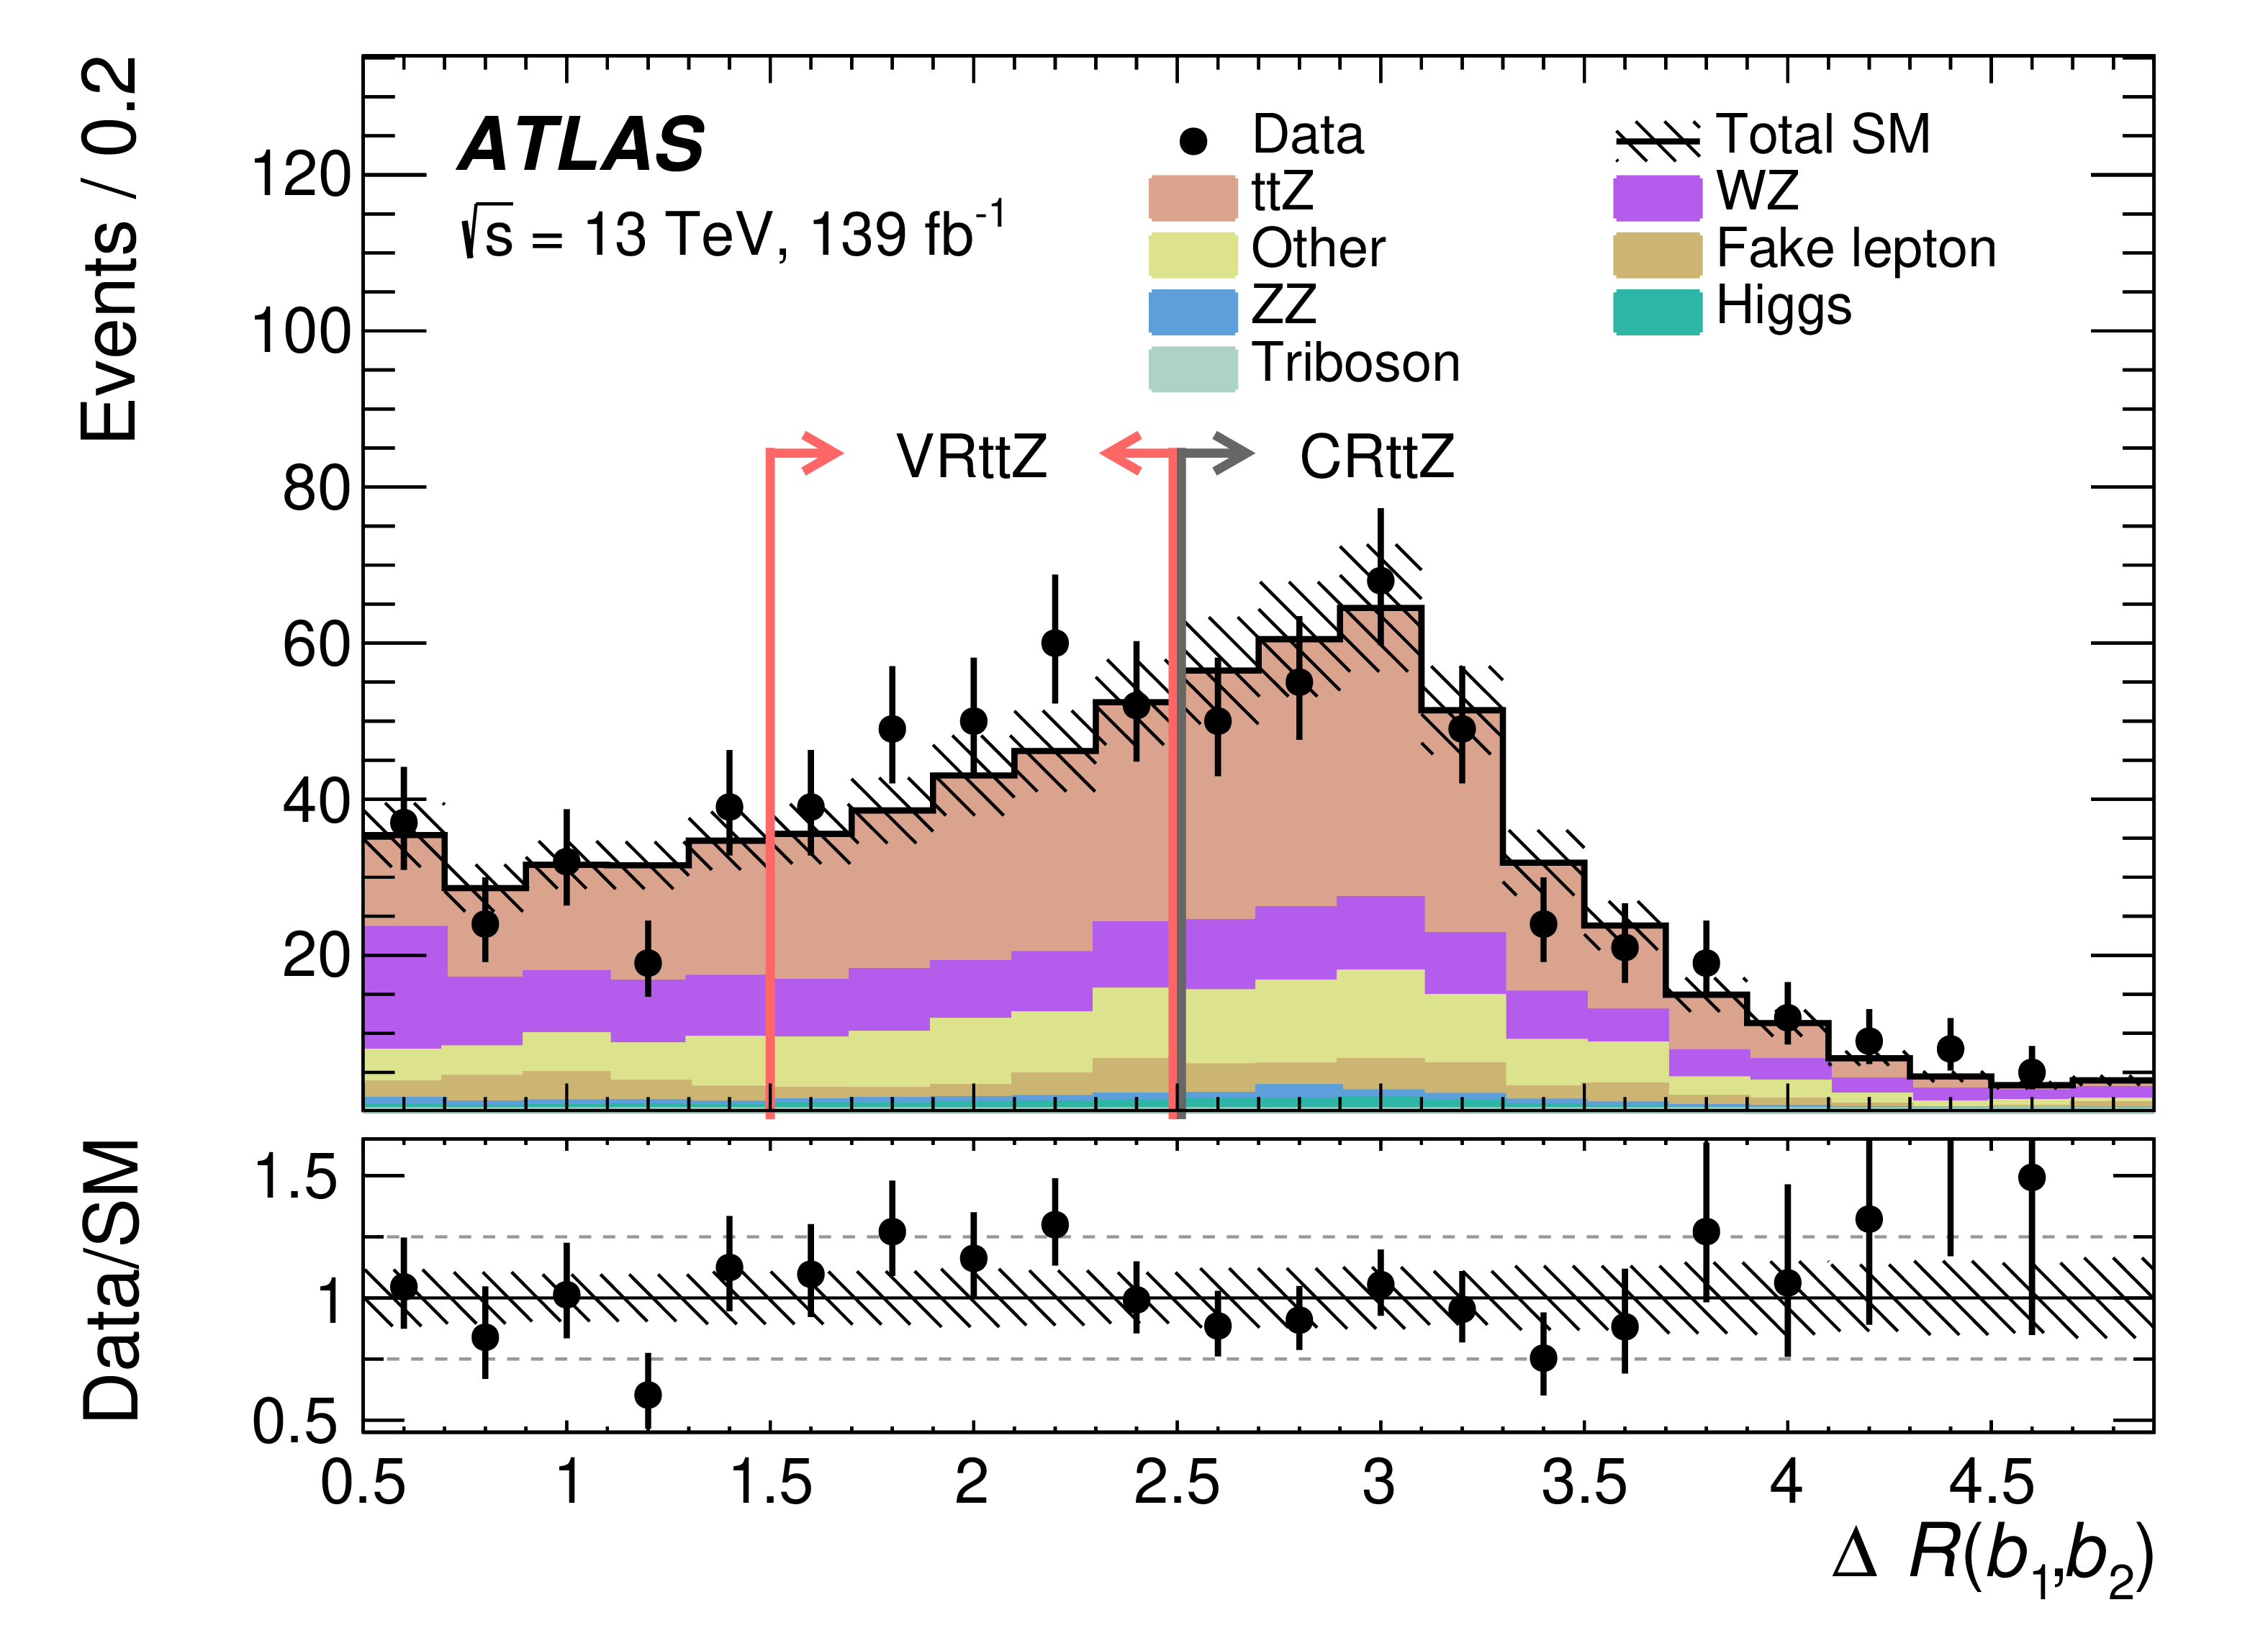
\includegraphics[width=0.98\textwidth]{figs/rpvthreel/CRttZ_Nm1_mydRbb.png}
      \caption{}
      \label{fig:Nminus1CRttZ}
    \end{subfigure}
    \caption[Distributions of the data and post-fit background in the CRs and VRs that are relevant in the extrapolation to the SRs (\mTmin in \CRWZ and \VRmTmin, \MET\ in \CRWZ, \MET\ in \VRmet, $m_{ll,2}$ in \CRZZ and \VRZZ, and \dRbb\ in \CRttZ and \VRttZ)]{Distributions of the data and post-fit background in the CRs and VRs that are relevant in the extrapolation to the SRs, including (top left) \mTmin in \CRWZ and \VRmTmin, (top right) \MET\ in \CRWZ, (middle left) \MET~ in \VRmet, (middle right) $m_{ll,2}$ in \CRZZ and \VRZZ, and (bottom) \dRbb in \CRttZ and \VRttZ. Black (red) arrows indicate the CR (VR) selection on the variable shown, with all other region selections applied~\cite{ATLAS:2020uer}.}
    \label{fig:postfitkinematics}
\end{figure}

\begin{figure}[tbp]
  \begin{center}
    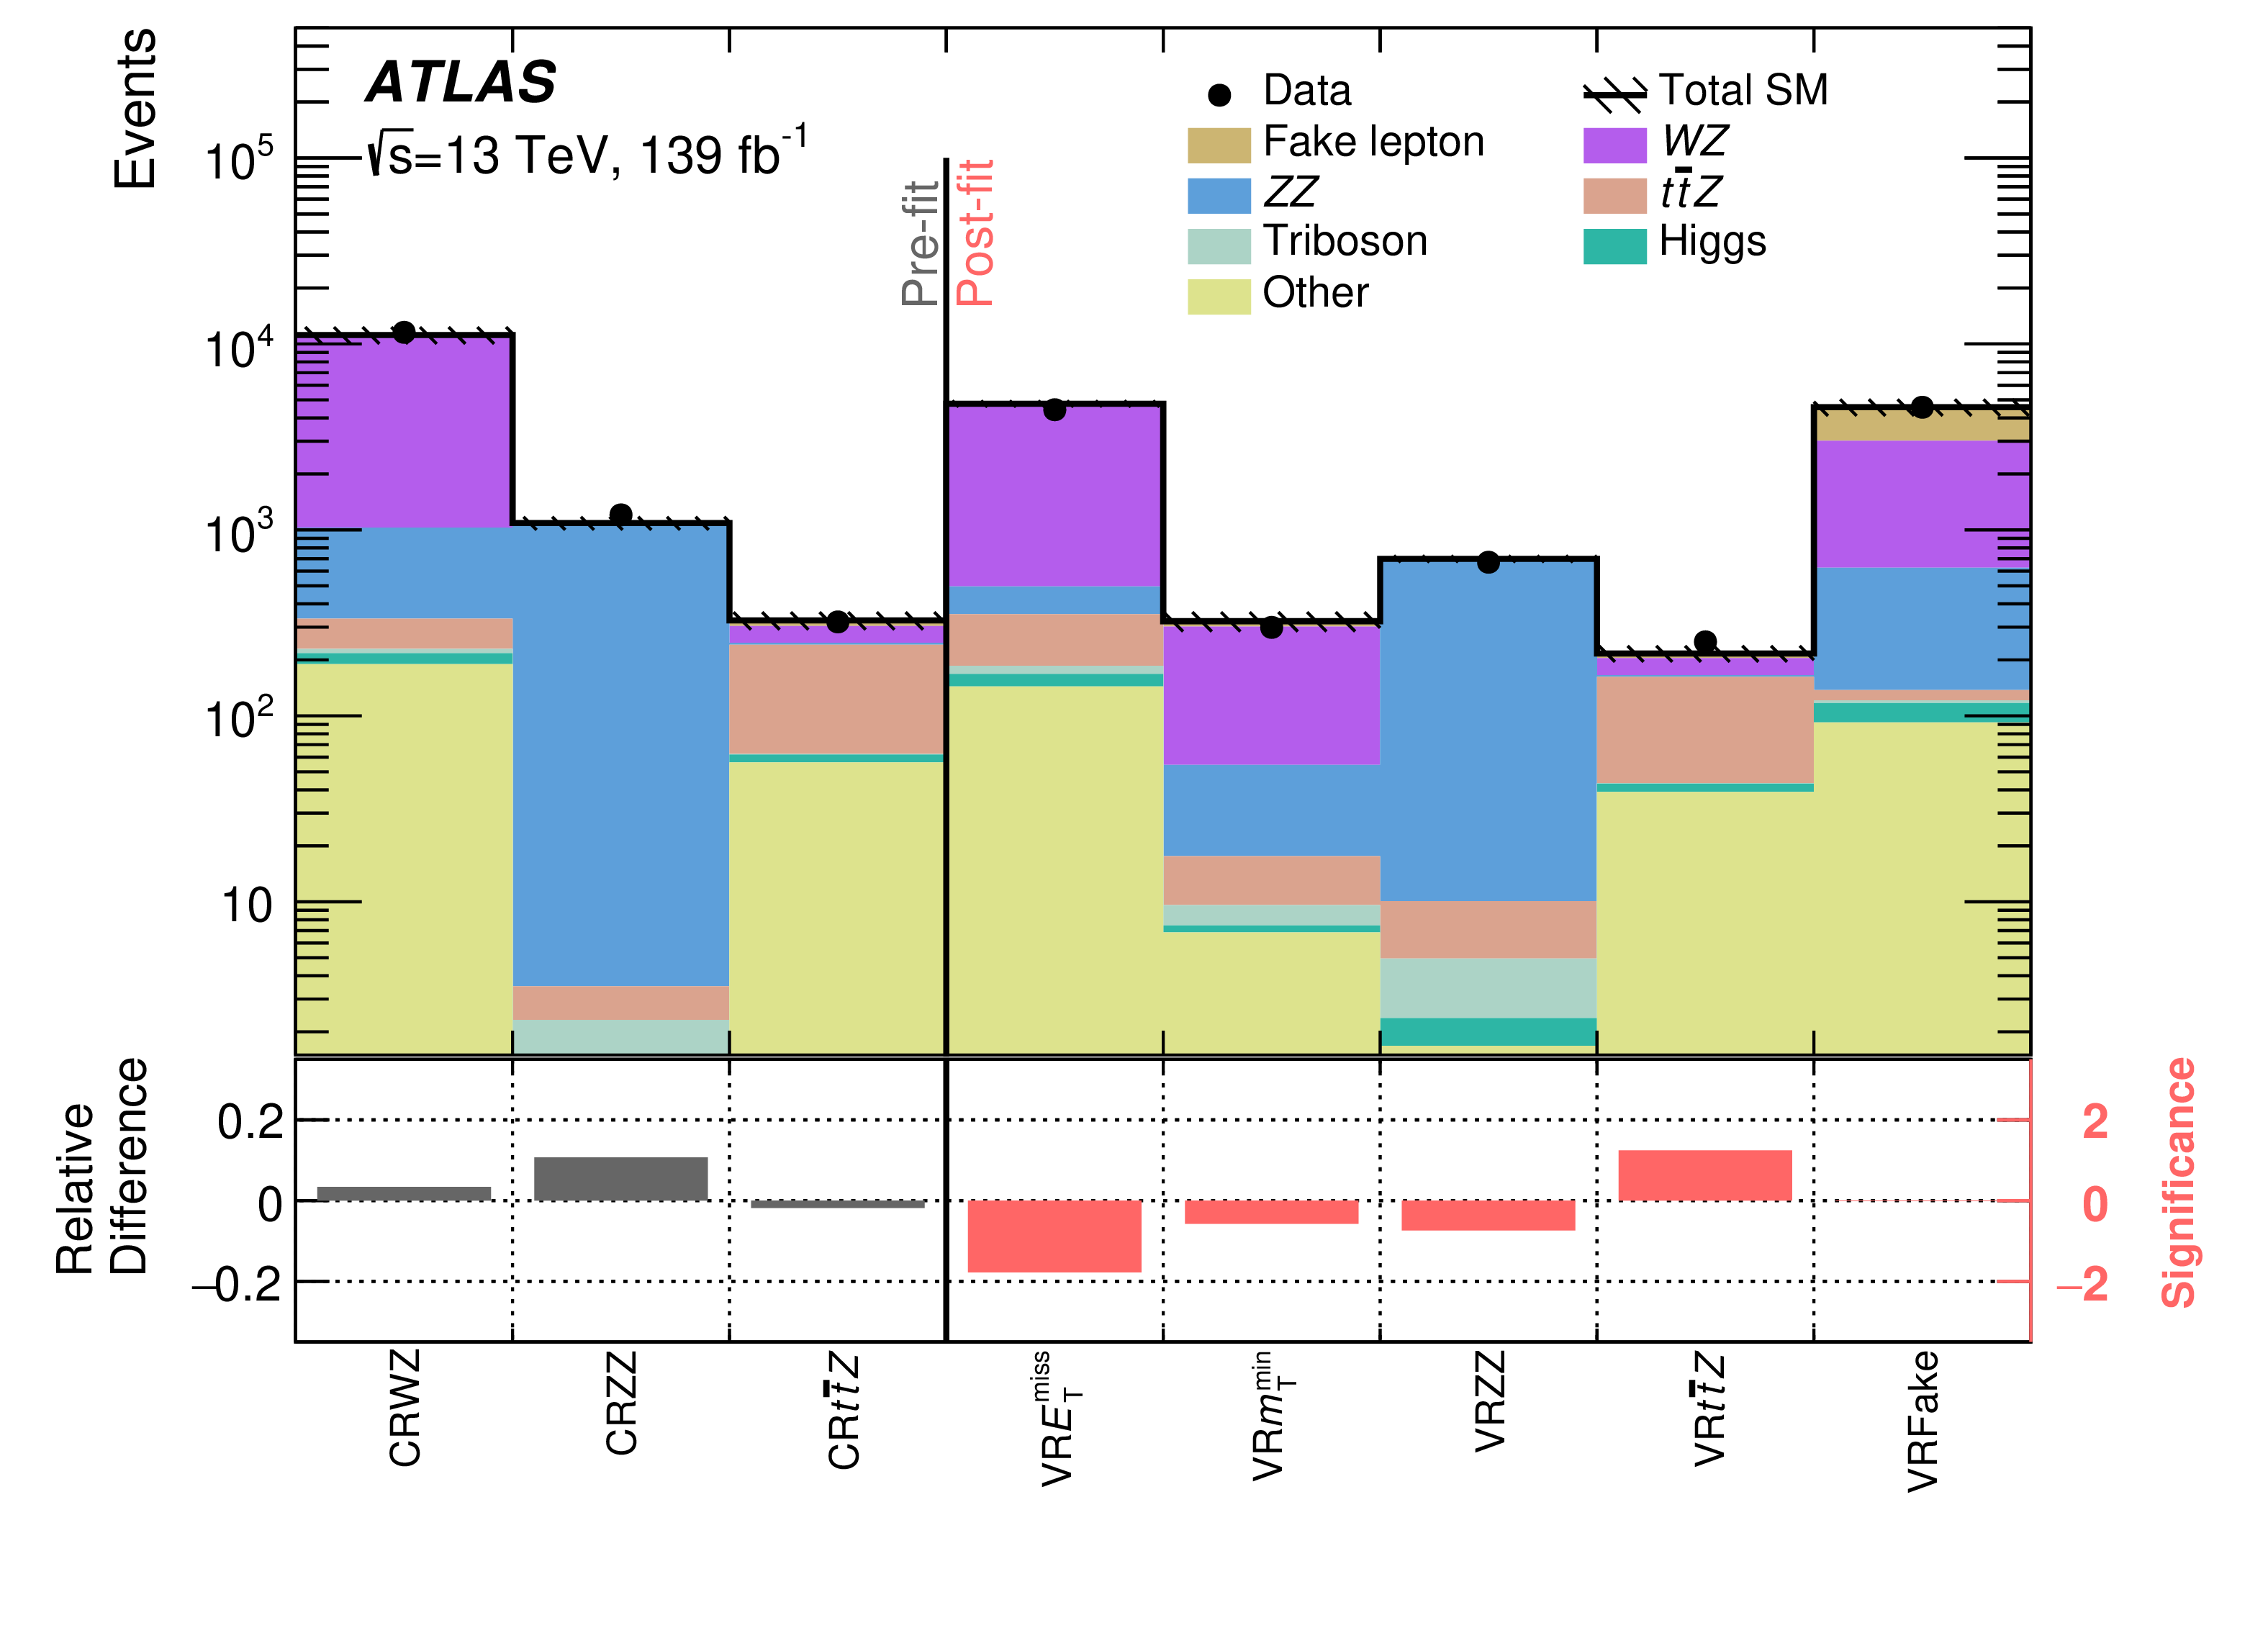
\includegraphics[width=0.98\textwidth]{figs/rpvthreel/histpull_all_doSRsInBkg_CRVR.png}
  \end{center}
  \caption[The observed data and the SM background expectation in the CRs (pre-fit) and VRs (post-fit).]
           {The observed data and the SM background expectation in the CRs (pre-fit) and VRs (post-fit). The ``Other'' category consists mostly of the \tWZ, \ttW, and \tZ processes. The hatched bands indicate the combined theoretical, experimental, and MC statistical uncertainties in the background prediction. The bottom panel shows the fractional difference between the observed  data and expected yields for the CRs and the significance of the difference for the VRs, computed following the profile likelihood method described in Sections \ref{sec:stats:MLE} and \ref{sec:stats:LikelihoodRatio}.}
   \label{fig:dataMCagreement_CRVR}
\end{figure}
%N-1 post-fit distributions are shown in Figure \ref{}

\subsection{Model Independent Fit}
\label{sec:stats:modind}

This fit considers one SR at a time, to avoid any assumption on relative signal contributions across SRs and \mZl bins.
Hence, this analysis has 48 discovery regions that are fit one-by-one in separate fits, corresponding to the 16 bins in each of the three SR types.

\subsection{Model Dependent Fit}
\label{sec:stats:moddep}
The second type of fit now includes the signal model contributions to the MC estimate. 
Each bin of the \mZl distribution in each SR is fit simultaneously.
By re-weighting the truth decays of the \chono, a scan over model branching ratio schemas, in addition to the nominal mass scan, is done to set limits for a large swath of model parameter space.
The granularity and technical specifications of this scan is described in detail in Section \ref{sec:BRscan}.







%While each region targets specific \chono decay chains, events in which one or more leptons fall outside the detector acceptance or are not reconstructed may still be selected by other regions.
%For the signal sample with a mass of 500~\GeV and democratic \chono branching fractions to bosons and leptons, the \SRTL, \SRFour, and \SRThree regions have selection efficiencies of 3\%, 4\%, and 5\%, respectively.
